\documentclass[research]{BMSTU-IU8}

\usepackage{amssymb} % triangleeq
\usepackage{pdfpages}

\student{Железцов Н.В.}
\theme{Анализ и формальная верификация алгоритма консенсуса Raft}
\group{ИУ8-94}

\supervisor{Колесников А.В.}

% \theme{Тест \hfill} % Тема для НИРСа заполняется по-другому
\studentFullName{Железцов Никита Владимирович}
\profile{20У474}
\speciality{10.05.01 <<Компьютерная безопасность>>}
\specialization{10.05.01\_01 <<Математические методы защиты информации>>}

\newacronym{bd}{БД}{База данных.}
\newacronym{subd}{СУБД}{Система управления базами данных.}
\newacronym{ddl}{DDL}{Data Definition Language.}
\newacronym{dql}{DQL}{Data Query Language.}
\newacronym{dml}{DML}{Data Manipulation Language.}
\newacronym{dcl}{DCL}{Data Control Language.}
\newacronym{lsn}{LSN}{Log sequence number.}
\newacronym{id}{ID}{Identifier.}
\newacronym{uuid}{UUID}{Universally unique identifier.}


\newglossaryentry{id1}{
    name={База данных (БД)},
    description={это организованная коллекция данных, которая структурирована таким образом, чтобы данные можно было легко хранить, управлять, изменять и извлекать.},
}

\newglossaryentry{id7}{
    name={Бакет},
    description={это логический контейнер, в который помещаются данные для
    распределения по шардам (физическим серверам или узлам). Это абстракция,
    которая связывает ключ шардирования с конкретным шардом.}
}

\newglossaryentry{id6}{
    name={Кластер},
    description={это совокупность нескольких репликасетов, каждый из которых чаще всего хранит разный набор данных.}
}

\newglossaryentry{id11}{
    name={Ребалансировка},
    description={процесс перевозки бакетов с одного шарда на другой.}
}

\newglossaryentry{id5}{
    name={Репликасет (replicaset, набор реплик, шард)},
    description={это группа узлов, работающих в режиме репликации и объединенных для обеспечения отказоустойчивости и доступности данных.}
}

\newglossaryentry{id2}{
    name={Система управления базами данных (СУБД)},
    description={это программное обеспечение, предназначенное для создания, управления и обеспечения доступа к базам данных. Оно позволяет пользователям определять, создавать, изменять и управлять базой данных, а также обеспечивает взаимодействие между пользователями и базой данных через запросы и команды. Основные функции включают хранение, поиск, обновление и удаление данных, а также обеспечение целостности, безопасности и управления доступом к данным.}
}

\newglossaryentry{id4}{
    name={Спейс (space)},
    description={это основная логическая единица хранения данных Tarantool, аналогичная таблице в традиционных реляционных базах данных. Спейс содержит набор записей, каждая из которых называется кортежем (tuple). Структура спейса определяется схемой, которая включает количество и типы полей в кортежах, а также индексы для быстрого доступа к данным.}
}

\newglossaryentry{id10}{
    name={Шардирование},
    description={это принцип проектирования базы данных, при котором данные
    разбиваются на части и размещаются на разных наборах реплик (репликасеты,
    шарды).}
}

\newglossaryentry{id8}{
    name={LSN},
    description={это монотонно возрастающий идентификатор записи.}
}

\newglossaryentry{id9}{
    name={Vclock},
    description={это массив LSN, идентификаторами в котором являются ID узлов. Vclock представляет собой набор логических счетчиков для каждого узла в кластере, позволяя определить, какие изменения были применены на конкретном узле и какие еще предстоит синхронизировать.}
}


\addbibresource{report.bib}

\begin{document}
    % \maketitle % Титульный лист

    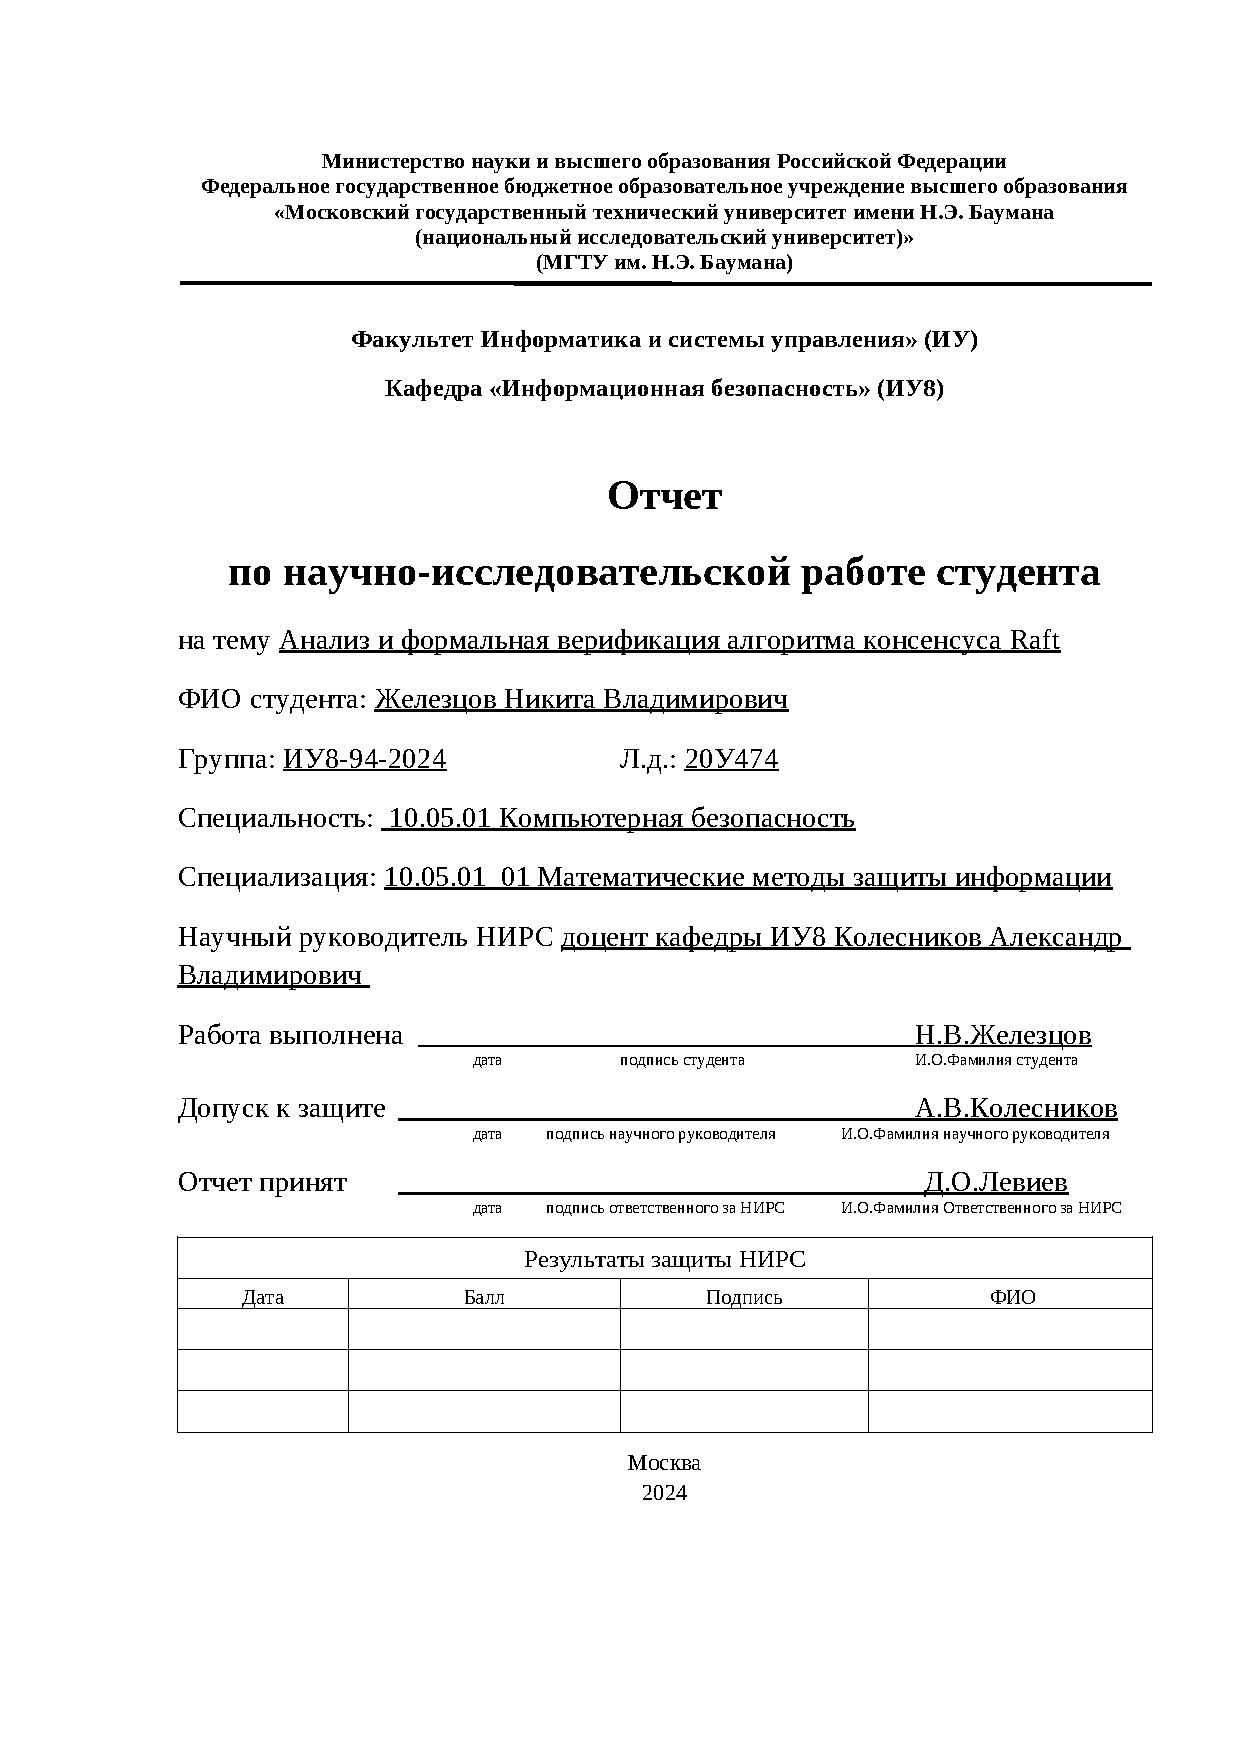
\includepdf[pages=-]{inc/titul.pdf} % Задание
    \setcounter{page}{4} % Устанавливает счётчик страниц

    \structure{РЕФЕРАТ}

Алгоритм Шора серьёзно поставил под вопрос безопасность информации, основанную
на криптосистемах с открытым ключом. Однако для взлома широко используемой
схемы RSA-2048 требуются миллионы физических кубитов, что значительно превышает
текущие технические возможности. Здесь мы сообщаем об универсальном квантовом
алгоритме факторизации целых чисел, объединяющем классическую редукцию базиса
решетки с квантовым алгоритмом приближённой оптимизации (QAOA). Количество
требуемых кубитов равно $O(\log N / \log\log N)$, что сублинейно относительно
битовой длины целого числа $N$, делая этот алгоритм самым экономичным по числу
кубитов алгоритмом факторизации на сегодняшний день. Мы экспериментально
демонстрируем алгоритм, факторизуя целые числа размером до 48 бит с помощью 10
сверхпроводящих кубитов, что является наибольшим целым числом, факторизованным
на квантовом устройстве. Мы оцениваем, что квантовая схема с 372 физическими
кубитами и глубиной в тысячи операций необходима для того, чтобы бросить вызов
RSA-2048 при помощи нашего алгоритма. Наше исследование демонстрирует
значительные перспективы для ускорения применения текущих шумных квантовых
компьютеров и прокладывает путь к факторизации больших целых чисел, имеющих
реальное криптографическое значение.
 % Реферат

    \tableofcontents % Содержание
    % \termsanddefenitions % Термины и определения
    % \listofabbreviations % Перечень сокращений и обозначений

    \structure{ВВЕДЕНИЕ}

Квантовые вычисления вступили в эпоху шумных квантовых устройств промежуточного
масштаба (NISQ) \cite{cite_1, cite_2}. Важной задачей эпохи NISQ является
демонстрация того, что устройства NISQ могут превзойти классические компьютеры
при решении задач с практической значимостью, то есть достижение практического
квантового преимущества. Алгоритмы, требующие минимальных ресурсов и
использующие ограниченное число доступных кубитов и глубину схем для решения
задач, сложных для классических вычислений, имеют особую важность. Вариационные
квантовые алгоритмы, использующие гибридную схему вычислений
«классика+квантовые вычисления», обладают значительным потенциалом для
получения значимого квантового преимущества в эпоху NISQ \cite{cite_3, cite_4,
cite_2, cite_5, cite_6}. Одним из таких алгоритмов является квантовый алгоритм
приближённой оптимизации (QAOA) \cite{cite_5}, первоначально предложенный для
решения задач на собственные значения, который впоследствии широко применялся в
различных областях, таких как химическое моделирование \cite{cite_7, cite_8},
машинное обучение \cite{cite_9}, а также инженерные приложения \cite{cite_10,
cite_11}.

Факторизация целых чисел является одной из важнейших основ современной
информационной безопасности \cite{cite_12}. Экспоненциальное ускорение
факторизации алгоритмом Шора \cite{cite_13} является выдающимся примером
превосходства квантовых вычислений. Однако выполнение алгоритма Шора на
отказоустойчивом квантовом компьютере требует значительных ресурсов
\cite{cite_14, cite_15}. На сегодняшний день наибольшее целое число,
факторизованное алгоритмом Шора на существующих квантовых системах, это число
21 \cite{cite_16, cite_17, cite_18}. Альтернативно, факторизация целых чисел
может быть сведена к задаче оптимизации, решаемой посредством адиабатических
квантовых вычислений (AQC) \cite{cite_19, cite_20, cite_21, cite_22} или QAOA
\cite{cite_23}. Более крупные числа были факторизованы этими методами на
различных физических системах \cite{cite_24, cite_25, cite_26, cite_27}.
Максимальные числа, факторизованные на данный момент, включают 291311 (19 бит)
в системе NMR \cite{cite_26}, 249919 (18 бит) на квантовом отжигателе D-Wave
\cite{cite_25}, 1099551473989 (41 бит) на сверхпроводящем устройстве
\cite{cite_27}. Однако следует отметить, что некоторые из факторизованных чисел
были специально подобраны с особыми структурами \cite{cite_28}, поэтому
наибольшее число, факторизованное универсальным методом на реальной физической
системе, на сегодняшний день составляет 249919 (18 бит).

В данной работе мы предлагаем универсальный квантовый алгоритм факторизации
целых чисел, требующий лишь сублинейные квантовые ресурсы. Алгоритм основан на
классическом алгоритме Шнорра \cite{cite_29, cite_30}, использующем редукцию
базиса решётки для факторизации целых чисел. Мы используем QAOA для оптимизации
наиболее трудоёмкой части алгоритма Шнорра, что ускоряет общее время
факторизации. Для целого числа $N$, имеющего $m$ бит, количество требуемых
кубитов в нашем алгоритме составляет $O(m / \log m)$, что сублинейно
относительно битовой длины числа $N$. Это делает наш алгоритм наиболее
экономным по числу кубитов по сравнению с существующими алгоритмами, включая
алгоритм Шора. С использованием данного алгоритма нами успешно факторизованы
числа 1961 (11 бит), 48567227 (26 бит) и 261980999226229 (48 бит) с
использованием, соответственно, 3, 5 и 10 кубитов на сверхпроводящем квантовом
процессоре. Число в 48 бит (261980999226229) также является наибольшим целым
числом, факторизованным универсальным методом на реальном квантовом устройстве.
Далее мы оцениваем квантовые ресурсы, необходимые для факторизации RSA-2048.
Согласно нашим расчётам, квантовая схема с 372 физическими кубитами и глубиной
порядка тысяч операций необходима для факторизации RSA-2048 даже в самой
простой одномерной системе. Подобный масштаб квантовых ресурсов, вероятно,
станет достижимым на устройствах NISQ в ближайшем будущем.

 % Введение

    \structure{ОСНОВНАЯ~ЧАСТЬ}

В первой части задается основа для последующего анализа алгоритмов консенсуса,
определяются термины распределенной системы и консенсуса, задаются условия и
ограничения, в которых эти алгоритмы могут быть применены.

Во второй части приводится описание алгоритма консенсуса Paxos, в третьей - Raft.
Оба этих алгоритма выполняются в распределенной системе, описанной в первой части.

В четвертой же части дается определение TLA+, проводится формальная верификация
алгоритма консенсуса Raft, строится модель система и производится ее проверка.

\section{Модель распределенной системы}

Формального определения распределенной вычислительной системы в настоящее время
не существует. Из множества различных определений, можно выделить ироничное
определение Лесли Лампорта, которое он дал в мае 1987 года,
в своем письме коллегам по поводу очередного отключения электроэнергии в машинном
зале:

«Распределенной вычислительной системой можно назвать такую систему, в которой
отказ компьютера, о существовании которого вы даже не подозревали, может сделать
ваш собственный компьютер непригодным к использованию».

Эндрю Таненбаум предложил следующее, более серьзное, определение
\cite{tanenbaum_distributed_systems}:

«Распределенная вычислительная система (РВС) – это набор соединенных каналами
связи независимых компьютеров, которые с точки зрения пользователя некоторого
программного обеспечения выглядят единым целым».

Именно это определение и будет использоваться в данной работе. Таким образом,
в РВС есть несколько автономных участников (иногда называемых процессами, узлами
или репликами). Каждый участник обладает своим локальным состоянием. Участники
выполняют некий алгоритм, общаются, обмениваясь сообщениями через каналы связи
между ними. Вне системы существуют пользователи, которые могут отправлять запросы
к различным узлам системы и ожидать от них ответов.

\subsection{Модель каналов связи}

Связь через каналы часто ненадежна: сообщения могут теряться, задерживаться или
приходить в неправильном порядке. В качестве отправной точки взят канал с
приемлемыми потерями (fair-loss) \cite{cachin11}:

\begin{itemize}
    \item Допустимые потери. Если отправитель и получатель функционируют корректно и
        процесс отправляет сообщение бесконечно много раз, оно в конечном итоге
        будет доставлено бесконечное число раз.
    \item Ограниченное дублирование. Одно отправленное сообщение не будет доставлено
        бесконечное количество раз.
    \item Без создания. Канал не создает новых сообщений, то есть доставляются
        только те сообщения, которые были отправлены.
\end{itemize}

Канал с приемлемыми потерями является полезной абстракцией и первым строительным
блоком для протоколов обмена данными с сильными гарантиями. По своей сути он похож
на протокол UDP, который позволяет отправлять сообщения от одного процесса другому,
но не предлагает надежной семантики доставки на уровне протокола. Однако гарантии,
предоставляемые такой моделью недостаточны для построения надежных распределенных
систем.

Для повышения надежности связи можно использовать подтверждения (acknowledgement,
ACK), позволяющие получателю уведомить отправителя о доставке сообщения. Для
этого применяются полнодуплексные каналы связи и добавляются механизмы,
которые помогают различать сообщения, например, уникальные порядковые номера
(sequence numbers), монотонно возрастающие идентификаторы.

До тех пор, пока отправитель не получит подтверждение о доставке сообщения,
он не может быть уверен, было ли оно обработано, будет ли обработано в будущем,
утеряно, либо удаленный процесс вышел из строя до его получения. Отправитель
может повторно передать сообщение, но это может вызвать его дублирование.
Безопасная обработка дубликатов возможна только в случае, если выполняемая
операция является идемпотентной. Поскольку в реальных условиях не всегда удается
обеспечить идемпотентность операций, требуется применять эквивалентные гарантии.
Для этого можно использовать методы дедупликации (deduplication), предотвращающие
повторную обработку одного и того же сообщения.

Повторные передачи и несоблюдение порядка доставки могут приводить к неверному
порядку поступления сообщений. Благодаря введению порядковых номеров получатель
может использовать их для восстановления порядка и обеспечения обработки сообщений
по принципу FIFO (first-in, first-out).

Применив все описанные выше ограничения к каналу с приемлемыми ограничениями,
получаем совершенный канал (perfect link), предоставляющий гарантии \cite{cachin11}:

\begin{itemize}
    \item Надежная доставка. Каждое сообщение, отправленное один раз корректным
        процессом А корректному процессу Б, в конце концов будет доставлено.
    \item Порядок сообщений. Сообщения будут доставлены в том порядке, в котором
        они были отправлены.
    \item Без дублирования. Ни одно сообщение не будет обработано более одного раза.
    \item Без создания. Канал доставляет только отправленные сообщения, не создавая
        новые.
\end{itemize}

Именно совершенный канал будет использоваться как модель канала для построения
алгоритмов коненсуса распределенных систем. Он похож на протокол TCP.

Однако даже совершенный канал не защищает алгоритм от ситуации разделения сети,
под которой понимается, что два или более процесса не могут связаться друг
с другом. Независимые группы процессов могут продолжать выполнение алгоритмов
и выдывать противоречивые результаты, могут происходить асимметричые отказы
каналов, при которых сообщения могут проходить только в одну сторону, но не
обратно. Все это необхоимо учитывать при разработке алгоритмов в распределенных
системах.

\subsection{Определение консенсуса}

Алгоритм консенсуса описывает работу распределенной системы, которая при наличии
нескольких процессов, начинающих работу с некого начального состояния, переводит
все процессы в одинаковое состояние. Чтобы алгоритм консенсуса был корректным,
должны выполняться следующие условия \cite{petrov}:

\begin{itemize}
    \item Согласованность. Принимаемое протоколом решение должно быть единодушным:
        каждый процесс  выбирает некоторое значение, которое должно быть
        одинаковым для всех процессов.
    \item Действительность. Согласованное значение должно быть предложено одним
        из процессов. Т.е. это не может быть некое произвольное значение.
    \item Окончательность. Согласованность принимает окончательный характер после
        того, как уже не остается процессов, не достигших состояния принятия решения.
\end{itemize}

\subsection{Теорема Фишера-Линча-Патерсона}

Мысленный эксперимент, известный как «задача двух генералов», наглядно
иллюстрирует сложности обеспечения консенсуса в распределенных системах.
Эксперимент демонстрирует, что в асинхронной системе, где нет временных
ограничений на доставку и ответы, невозможно достичь полного согласия между
сторонами, даже с использованием многочисленных подтверждений.

Суть задачи такова: две армии под командованием генералов расположены по разные
стороны от города и должны атаковать одновременно, чтобы достичь успеха.
Генералы передают сообщения через посланников, чтобы договориться об атаке.
Однако посланники могут быть перехвачены или не доставить сообщение, что
создает неопределенность. То есть генералам необходимо достичь консенсуса
по времени начала атаки.

Например, генерал А отправляет сообщение MSG(N), предлагая атаку в определенное
время. Генерал Б, получив сообщение, посылает подтверждение ACK(MSG(N)). На
рис. \ref{fig:generals} показано, что сообщение отправляется в одну сторону и
подтверждается  другой стороной.

\begin{figure}
  \centering
  \includegraphics[scale=0.4]{inc/generals.png}
  \caption{Задача двух генералов}
  \label{fig:generals}
\end{figure}

Однако генерал А не может быть уверен, что это подтверждение дошло, оно может
быть утеряно. Чтобы устранить сомнения, требуется второе подтверждение —
ACK(ACK(MSG(N))). Этот процесс может продолжаться бесконечно, поскольку всегда
остается риск того, что последнее сообщение не достигло адресата.

В задаче не сделано предположений о времени, не установлено лимита, за которое
генералы должны ответить, связь полностью асинхронна.

В работе Фишера, Линча и Патерсона рассматривается проблема, известная как
невозможность ФЛП (FLP Impossibility) \cite{fischer85}. Эта теорема, также
именуемая теоремой Фишера–Линча–Патерсона, изучает консенсус в системах, где
процессы начинают с начального значения и стремятся согласовать новое общее
значение. После выполнения алгоритма это значение должно быть одинаковым для
всех корректно работающих процессов.

В исследовании предполагается полностью асинхронная среда, где процессы не
имеют общего времени. Алгоритмы в таких системах не могут полагаться
на время ожидания, а у процесса отсутствует возможность определить, отказал ли
другой процесс или просто работает медленно. В статье доказывается, что при
указанных предположениях невозможно создать протокол, который гарантирует
достижение консенсуса за ограниченное время. Даже один сбой процесса, не
сопровождающийся уведомлением, делает консенсус недостижимым для полностью
асинхронной распределенной системы.

Тем не менее, теорема ФЛП не утверждает, что достижение консенсуса в принципе
невозможно. Она лишь показывает, что в асинхронной системе консенсус не всегда
достижим за конечное время. В реальных системах часто присутствует некоторая
степень синхронности, и эту особенность нужно учитывать.

\subsection{Синхронность}

Из теоремы ФЛП следует, что ключевой характеристикой распределенной системы
является предположение о времени. В асинхронных системах невозможно
гарантировать ограниченные задержки в доставке сообщений, упорядоченность их
получения. Процесс выдает ответ через неопределенной долгое время.

Однако, одним из аргументов против асинхронных систем является их оторванность
от реальности: процессы не имеют произвольно разные скорости обработки, а
задержки передачи сообщений не бывают бесконечными.

Можно сделать предположения менее строгими, считая систему синхронной. Может
предполагаться, что процессы работают с сопоставимыми скоростями, задержки
передачи сообщений в канале ограничены, их доставка не может занимать
бесконечно долгое время.

В модель синхронной системы также можно добавить локальные для процесса
синхронизированные часы: при этом существует некоторая верхняя граница в раз­
нице во времени между двумя локальными для процессов источниками времени
\cite{cachin11}.

Свойства асинхронных и синхронных моделей можно объединить, рассматривая
систему как частично синхронную. Частично синхронная система обладает некото­
рыми свойствами синхронной системы, но при этом ограничения на время доставки
сообщений, уход показаний часов и относительные скорости обработки могут быть
приблизительными и действовать лишь в большинстве случаев.

\subsection{Модели отказов}

Модель отказов описывает, каким образом могут происходить сбои в работе
процессов распределенной системы. Например, можно предположить, что процесс
может полностью завершить работу и не восстановиться, восстановиться через
некоторое время или начать выдавать некорректные данные из-за сбоя или
преднамеренно.

Поскольку процессы в распределенных системах взаимодействуют друг с другом
при выполнении алгоритма, сбои в одном из них могут нарушить выполнение всей
системы. Для разработки алгоритмов в распределенных системах необходимо понимать,
какие отказы могут случиться, чтобы правильно обрабатывать каждый из них.

\subsubsection*{Аварийное завершение}

В этой модели предполагается, что процесс перестает выполнять шаги алгоритма
и не отправляет сообщений другим процессам. После сбоя процесс остается в этом
состоянии и больше не участвует в текущем выполнении алгоритма.

Важно отметить, что эта модель не запрещает восстановление процессов. Процесс
может восстановиться, синхронизироваться с текущим состоянием системы и
участвовать в новых раундах алгоритма.

Процесс, который восстанавливается после сбоя, может продолжить выполнение с
последнего известного ему шага. Алгоритмы, поддерживающие восстановление,
должны вводить в систему понятия устойчивого состояния алгоритма и протокола
восстановления \cite{skeen83}.

\subsubsection*{Пропуск}

В этой модели процесс пропускает выполнение отдельных шагов алгоритма, либо
эти шаги невидимы для других участников, либо процесс не может отправлять и
получать сообщения. Пропуски включают сетевые сбои, вызванные неисправностями
каналов связи, отказами оборудования или перегрузкой сети.

Пропуски возникают, когда алгоритм не завершает определенные действия, или их
результаты не достигают других процессов. Например, потерянное сообщение может
привести к тому, что отправитель считает его доставленным, несмотря на его
окончательную утрату.

\subsubsection*{Византийские ошибки}

Произвольные, или византийские, ошибки (Byzantine faults) представляют собой
наиболее сложный класс отказов. В этом случае процесс продолжает выполнять шаги
алгоритма, но делает это некорректно.

Такие сбои могут быть вызваны ошибками в программном обеспечении, выполнением
разных версий алгоритма или намеренными действиями злоумышленников. Например,
в распределенных системах без централизованного управления, таких как
криптовалюты, процессы могут фальсифицировать данные, чтобы ввести систему в
заблуждение.

\subsubsection*{Обработка отказов}

Одним из способом обработки отказов при невизантийских ошибках является введение
в алгоритм избыточности. Таким образом отказ может быть замаскирован: даже если
один или несколько процессов откажут, то пользователь этого не заметит
\cite{christian91}. Raft и Paxos, которые будут рассмотрены в данной работе,
основываются на модели отказов и минимизирует влияение отказов путем
использования избыточности процессов.

В случае работы в распределенной системе с византийскими ошибками используется
перекрестная проверка других узлов на каждом шаге, поскольку узлы не могут
полагаться друг на друга или на лидера и должны проверять поведение других узлов,
сравнивая возвращаемые результаты с ответами большинства. PBFT, PoW, PoS борются
с ошибками именно так.

\subsection{Итоги}

Таким образом, к распределенной системе, в которой будет исполняться любой из
описанных в данной работе алгоритм консенсуса, применяются следующие ограничения:

\begin{itemize}
    \item Система передает сообщения по совершенным каналам, однако допустимо
        разделение сети.
    \item Необходимо учитывать возможность отказа узлов: аварийное завершение и
        пропуск части алгоритма процессом.
    \item В системе невозможны византийские ошибки. Предполагается, что все узлы
        честные и выполняют свои функции корректно.
    \item Система является частично синхронной, в ней существует понятие времени,
        которое используется для синхронизации локальных часов. Сообщения в системе
        могут отправляться бесконечно, процессы могут работать с произвольной
        скоростью.
\end{itemize}

    \section{Паксос}

Алгоритм Паксос (Paxos) считается одним из самых известных методов достижения
консенсуса. Его предложил Лесли Лэмпорт в своей работе The Part-Time
Parliament («Парламент с неполной занятостью») \cite{lamport98}. В данной
статье идея консенсуса была представлена через метафору законодательного
процесса и голосования, происходящих на острове Паксос. Позднее, в 2001 году,
Лэмпорт опубликовал статью Paxos Made Simple («Простой Паксос») \cite{lamport01},
где использовал упрощенную терминологию, которая и используется в данной работе.

В рамках алгоритма Паксос участники могут выполнять одну из трех ролей:

\begin{itemize}
    \item Заявители (proposers). Принимают значения от клиентов, формируют
        предложения для их утверждения и пытаются получить голоса акцепторов.
    \item Акцепторы (acceptors). Участвуют в голосовании за принятие или
        отклонение предложений, сформированных заявителями. Для устойчивости
        к отказам система включает несколько акцепторов, однако для принятия
        решения достаточно кворума (то есть большинства голосов).
    \item Ученики (learners). Отвечают за хранение результатов принятых решений,
        выполняя роль реплик.
\end{itemize}

В большинстве реализаций эти роли совмещены в одном процессе.

Каждое предложение содержит уникальный номер, который монотонно увеличивается,
и значение, предложенное клиентом. Номер предложения используется для установления
общего порядка операций и определения их последовательности («до» или «после»).
Номера предложений часто оформляются как пара (идентификатор узла и временная метка).
Идентификаторы узлов являются упорядочиваемыми и могут быть использованы для
разрешения конфликтов между временными метками. Для корректной работы алгоритма
требуется синхронизация локальных часов.

\subsection{Алгоритм Paxos}

Алгоритм Паксос можно разделить на два ключевых этапа: голосование (или этап
предложения) и репликацию. На этапе голосования заявители борются за установление
своего лидерства, а на этапе репликации заявитель распространяет согласованное
значение среди акцепторов.

Заявитель выступает как начальная точка контакта для клиента, получая значение,
которое должно быть принято, и пытается собрать голоса от акцепторов. После
этого акцепторы рассылают информацию о принятом значении среди учеников, что
позволяет ответить пользователю. Ученики, в свою очередь, увеличивают
коэффициент репликации согласованного значения.

Только один заявитель может получить большинство голосов. В случае, если
голоса распределяются равномерно, ни один из заявителей не сможет набрать
большинство, и тогда им придется начать процесс заново.

На этапе предложения заявитель отправляет запрос $Подготовка(n)$ (где $n$ —
номер предложения) большинству акцепторов, пытаясь собрать их голоса. Акцептор,
получив запрос, должен ответить, соблюдая несколько инвариантов \cite{lamport01}:

\begin{itemize}
    \item Если акцептор еще не отвечал на запрос с более высоким порядковым
        номером, он обещает не принимать предложения с меньшими номерами.
    \item Если акцептор уже принял какое-то предложение, он уведомляет
        заявителя о принятом значении через сообщение $Обещание(m, v_{\text{принятых}})$.
    \item Если акцептор ранее ответил на запрос с большим порядковым номером, он
        уведомляет заявителя о существующем предложении с более высоким номером.
    \item Акцептор может ответить на несколько запросов, если последний имеет
        наибольший порядковый номер.
\end{itemize}

Когда заявитель получает большинство голосов, начинается этап репликации.
Заявитель фиксирует предложение, отправляя акцепторам сообщение $Принятие(n, v)$,
где $v$ — это значение, соответствующее предложению с наибольшим номером среди
полученных ответов от акцепторов, или собственное значение заявителя, если
акцепторы не приняли других предложений.

Акцептор примет предложение с номером $n$, если на этапе предложения он не
ответил на запрос с большим номером. Если акцептор отклоняет предложение, он
отправляет заявителю максимальный порядковый номер, который он видел, для
актуализации данных заявителя \cite{lamport01}.

Обобщенная схема раунда Паксос приведена на рис \ref{fig:paxos}.

\begin{figure}
  \centering
  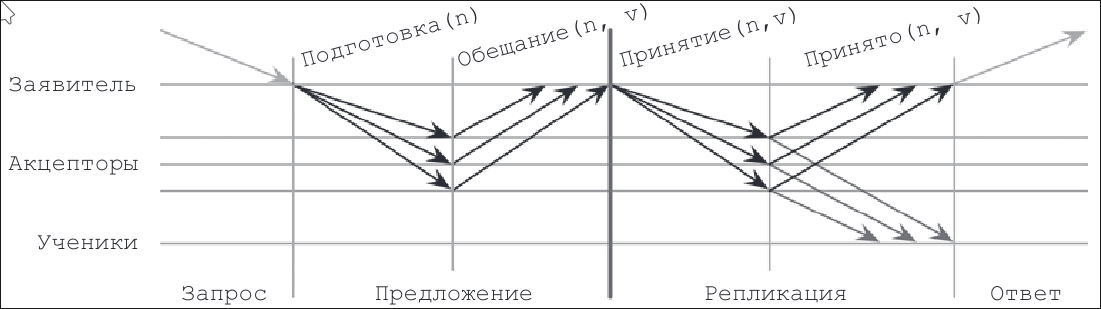
\includegraphics[scale=0.4]{inc/paxos.png}
  \caption{Схема раунда Паксос}
  \label{fig:paxos}
\end{figure}

После того как консенсус относительно значения достигнут (хотя бы один акцептор
принял решение), последующие заявители должны принять это значение, чтобы
сохранить согласованность. Поэтому акцепторы возвращают последнее принятое
значение. Если ни один акцептор не видел предыдущего значения, заявителю
разрешается выбрать собственное.

Ученики получают информацию о принятом значении, когда большинство акцепторов
сообщает им об этом. Акцепторы могут сразу уведомить учеников о принятом
значении. При наличии нескольких учеников акцепторы должны уведомить каждого,
однако можно выделить несколько учеников, которые будут отвечать за
уведомление других.

Таким образом, основной целью первого этапа алгоритма является установление
лидера и определение принятого значения, что позволяет перейти ко второму
этапу — распространению значения. В базовом алгоритме оба этапа выполняются
каждый раз, когда необходимо принять решение. Однако на практике можно
уменьшить количество шагов. Этот подход будет рассмотрен позже в разделе
"Мульти-Паксос".

\subsection{Мульти-Паксос}

Ранее мы рассматривали классический Паксос, в котором любой узел может стать
заявителем и инициировать раунд. Проблема этого подхода в том, что для каждого
нового раунда репликации требуется запускать стадию предложения (этап с
Подготовкой). Чтобы избежать таких повторений и дать заявителю возможность
многократно использовать своё положение, применяется мульти-Паксос \cite{lamport01}.
Он вводит роль лидера — выделенного заявителя, который после утверждения может
сразу приступать к репликации, минуя стадию предложения.

В классическом Паксосе чтение часто реализуется через дополнительный раунд,
собирающий любые незавершённые данные, поскольку нет гарантии, что последний
заявитель имеет самую свежую версию состояния. В мульти-Паксосе появляется
сходная проблема: если мы читаем данные у лидера, который уже успел смениться,
то можем получить устаревшую информацию. Чтобы этого избежать и поддерживать
линеаризуемость, некоторые реализации используют механизм аренды (lease)
\cite{chandra07}. Лидер периодически подтверждает свою активность, а узлы
обещают не принимать другие предложения в течение срока аренды. Этот приём не
гарантирует абсолютную корректность, но ускоряет операции чтения при условии
ограниченной синхронизации часов. Однако в случае рассинхронизации часов, когда
лидер считает, что его срок аренды не истек, а другие участники - наоборот,
линеаризуемость недостижима.

Мульти-Паксос обычно описывают как реплицируемый журнал операций над некоторой
структурой. При сбоях участники восстанавливают данные из долговременного журнала
сообщений. Чтобы журнал не разрастался бесконечно, принято периодически
создавать моментальные снимки состояния (снапшоты) и усекать журнал до отметки
этого снимка.

    \section{Raft}

На протяжении длительного времени для достижения консенсуса применялся алгоритм
Паксос, однако в кругах разработчиков распределённых систем он считался
чрезмерно сложным. В 2013 году был предложен новый подход под названием Raft,
ориентированный на упрощение понимания и реализации \cite{ongario14}.

В Raft каждый узел хранит локально журнал команд, исполняемых конечным автоматом.
Так как все процессы получают одинаковые входные данные и применяют идентичные
команды в одном и том же порядке, их конечные автоматы приходят к одинаковому
состоянию. Одно из отличий Raft заключается в том, что роль лидера здесь
вынесена на первый план: он координирует репликацию и манипуляции над конечным
автоматом. С этой точки зрения Raft схож с Мульти-Паксосом и атомарной рассылкой:
среди узлов выбирается лидер, который принимает решения и задаёт упорядочение
сообщений.

Алгоритм Raft определяет три основные роли:

\begin{itemize}
    \item Кандидат (candidate): Узел, который пытается стать лидером. Он набирает
        голоса большинства узлов. Если выборы не приводят к явному победителю,
        запускается новый период и процесс голосования повторяется.
    \item Лидер (leader): Временный управляющий кластером, обрабатывающий запросы
        клиентов и взаимодействующий с реплицируемым конечным автоматом. Лидер
        выбирается на определённый период, который идентифицируется возрастающим
        номером. Если лидер перестаёт отвечать или подозревается в отказе,
        начинается процедура переизбрания.
    \item Последователь (follower): Пассивный участник, хранящий записи журнала
        и реагирующий на запросы от лидера и кандидатов. По сути, в Raft он
        объединяет в себе функции акцептора и ученика из Паксоса. Каждый узел
        стартует в роли последователя.
\end{itemize}

Чтобы добиться упорядочения без жёсткой синхронизации часов, в Raft используются
периоды (эпохи, термы), в течение которых существует только один лидер. Каждый
период имеет уникальный номер, а команды внутри периода получают дополнительный
индекс. Узлы могут по-разному воспринимать текущий период (например, если они
пропустили этап выборов), но каждая отправляемая команда указывает номер
периода \cite{ongario14}. Если узел видит период с более высоким номером, он
обновляет своё значение периода.

Процесс выбора лидера инициируется, когда последователь не получает подтверждений
от текущего лидера, полагая, что тот вышел из строя. В этом случае последователь
переходит в состояние кандидата и собирает голоса большинства узлов, стремясь
стать новым лидером.

На рис. \ref{fig:raft} приведена схема раунда Raft.

\begin{figure}
  \centering
  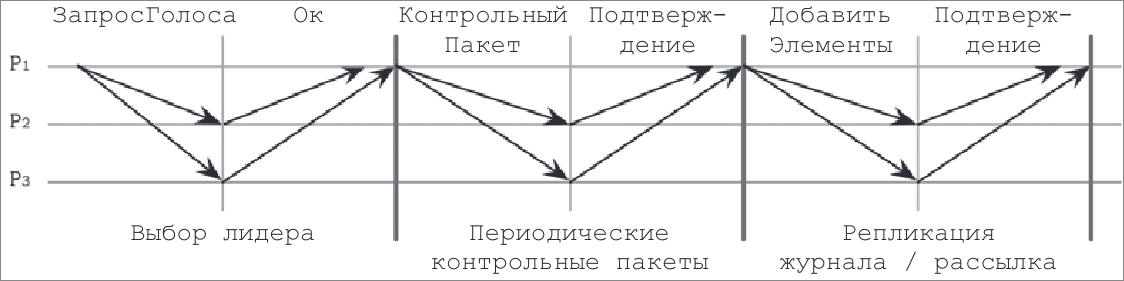
\includegraphics[scale=0.4]{inc/raft.png}
  \caption{Схема раунда Raft}
  \label{fig:raft}
\end{figure}

\begin{itemize}
    \item Выбор лидера. Когда узел-кандидат (P1 на рисунке) решает стать лидером,
        он рассылает остальным участникам сообщение $ЗапросГолоса$, содержащее свой
        период, последнюю известную ему информацию о периоде, а также идентификатор
        самой свежей записи в журнале, которую он видел. Если кандидат получает
        большинство голосов, он становится лидером на текущий период. При этом
        каждый узел может отдать голос лишь одному кандидату.
    \item Периодические контрольные пакеты. Для поддержания жизнеспособности
        системы лидер с определённой периодичностью отправляет контрольные
        пакеты всем последователям, тем самым подтверждая своё лидерство. Если
        последователь не получает такие пакеты в течение «тайм-аута выборов»,
        он предполагает сбой лидера и инициирует новый процесс голосования.
    \item Репликация. Лидер может неоднократно пополнять реплицируемый журнал,
        отправляя сообщение $ДобавитьЭлементы$, где указывает период лидера,
        индекс и период последней зафиксированной записи, а также одну или
        несколько новых записей для сохранения.
\end{itemize}

\subsection{Роль лидера в Raft}

Лидер может быть выбран только среди узлов, содержащих все актуальные записи.
Если в процессе выборов журнал последователя более актуальный, чем у кандидата,
то голос за этого кандидата не отдается.

Для победы в голосовании кандидат должен получить большинство голосов. Поскольку
записи реплицируются строго по порядку, достаточно сравнить идентификаторы последних
записей. После избрания лидер начинает принимать запросы от клиентов и реплицирует
их на своих последователей. Для этого он добавляет запись в свой журнал и
одновременно отправляет её всем последователям.

Когда последователь получает сообщение о добавлении записей, он вносит эти
записи в локальный журнал и отправляет подтверждение, сообщая лидеру, что данные
сохранены. Как только лидер получает достаточное количество подтверждений, запись
считается зафиксированной и помечается соответствующим образом в его журнале.

Поскольку лидером может стать только узел с наиболее актуальными данными,
последователь не отправляет ему обновления. Записи журнала передаются
только в одном направлении — от лидера к последователям.

\begin{figure}
  \centering
  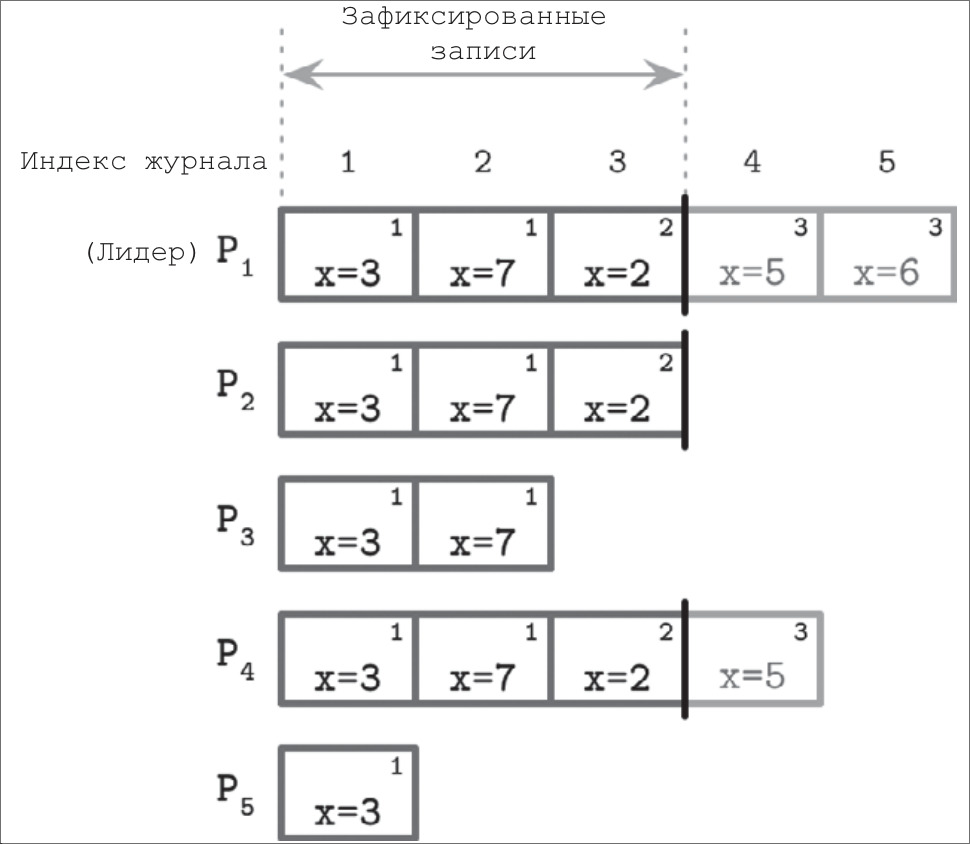
\includegraphics[scale=0.4]{inc/raft-consensus.png}
  \caption{Конечный автомат алгоритма Raft}
  \label{fig:raft-consensus}
\end{figure}

На рисунке \ref{fig:raft-consensus} представлен пример раунда достижения
консенсуса, в котором узел P1 выступает в роли лидера с наиболее актуальной
информацией. Лидер выполняет алгоритм, реплицируя записи на своих последователей
и фиксируя их после получения подтверждений. Фиксация одной записи автоматически
фиксирует все предшествующие записи в журнале. Решение о фиксации может принимать
только лидер. Каждая запись в журнале имеет идентификатор периода (терма, указан в
верхнем правом углу записи) и индекс, определяющий её позицию в журнале.
Зафиксированные записи гарантированно реплицируются на кворум узлов, что
позволяет безопасно применять их к конечному автомату в порядке их добавления.

\subsection{Сценарии отказов}

Когда несколько последователей решают стать кандидатами, но ни один из них не
может набрать большинство голосов, такая ситуация называется "разделенным
голосованием". Чтобы снизить вероятность таких случаев, алгоритм Raft применяет
рандомизированные таймеры. Это позволяет одному из кандидатов начать следующий
этап выборов раньше других, получить достаточное количество голосов и быть
избранным, пока остальные кандидаты находятся в ожидании. Такой подход ускоряет
процесс выборов, исключая необходимость дополнительной координации между кандидатами.

Если последователи отключаются или задерживают ответы, лидер обязан
предпринимать дополнительные попытки доставки сообщений. Если подтверждение от
узлов не поступает в ожидаемый срок, лидер повторно отправляет сообщения.

Благодаря уникальным идентификаторам, присваиваемым реплицируемым записям,
порядок в журнале остается неизменным, даже при повторной доставке сообщений.
Последователи устраняют дублирующие записи, основываясь на их порядковых номерах,
что предотвращает нежелательные эффекты от повторных отправок. Также порядковые
номера используются для соблюдения хронологии в журнале: последователь отклоняет
записи с более высокими номерами, если предыдущие записи не совпадают с
его журналом. Если две записи из разных журналов имеют одинаковые идентификаторы
и индексы, то они хранят одну и ту же команду, а все предшествующие им записи
идентичны.

Для обнаружения сбоев лидер отправляет последовательным узлам контрольные
сообщения, подтверждая тем самым активность своего периода. Если один из узлов
замечает, что текущий лидер перестал отвечать, он инициирует процедуру выборов.
Новый лидер восстанавливает состояние кластера, определяя последнюю согласованную
запись (то есть запись с наибольшим номером, которую разделяют лидер и последователь).
Он приказывает узлам удалить все незафиксированные записи после этой точки и
реплицирует актуальные записи из своего журнала. Лидер не удаляет и не
перезаписывает собственные записи, а только добавляет новые.

Таким образом, Raft предоставляет следующие гарантии:

\begin{itemize}
    \item Только один лидер может быть избран одновременно на заданный период (терм);
        в течение одного периода не может быть двух активных лидеров;
    \item Лидер не удаляет и не переупорядочивает содержимое журнала; он только
        добавляет новые сообщения к нему;
    \item Зафиксированные записи в журнале гарантированно присутствуют в журналах
        для последующих лидеров;
    \item Все сообщения однозначно идентифицируются по идентификаторам сообщений
        и периодов; ни текущий, ни последующие лидеры не могут повторно использовать
        один и тот же идентификатор для другой записи.
\end{itemize}


    \include{contents/2-04-comparison.tex}
    \section{Реализация алгоритма Raft на TLA+}

TLA+ — язык спецификаций, основанный на теории множеств, логике первого порядка
и темпоральной логике действий (англ. TLA, temporal logic of actions).

Темпоральная логика была введена Амиром Пнуэли в 1970-х годах \cite{amir70}.
Лесли Лэмпорт увидел недостаточность этой идеи для описания систем целиком и
пришёл к мысли о необходимости использовать конечные автоматы, которым
придавался смысл формул темпоральной логики, описывающих все возможные
пути исполнения. Таким образом родилась идея темпоральной логики действий
(TLA), которая дополнила темпоральную логику следующим \cite{lamport08}:

\begin{itemize}
    \item инвариантность при повторении состояния;
    \item темпоральное использование кванторов существования;
    \item принятие в качестве атомарных формул не только предикатов состояния,
        но и формул действий.
\end{itemize}

TLA-спецификация — темпоральная формула, часто называемая $Spec$ и являющаяся
предикатом (утверждением) о поведении. Поведение представляет собой возможный
путь исполнения системы \cite{habrias06}.

Состоянием называется присваивание значений переменных, шагом называется пара
состояний. Теперь поведение можно представить как бесконечную последовательность
состояний, а шагами поведения можно назвать пару последовательных состояний
поведения. Предикатом состояния называется функция, результат которой —
логическое значение истина или ложь — соответствует утверждению о состоянии.
Действием называется функция, имеющая смысл предиката над шагом. В этой функции
участвуют как переменные первого шага, так и второго, которые обычно
отмечаются штрихом \cite{habrias06}.

$$
Spec \triangleq Init \wedge \Box [Next]_{(v_1, v_2, ..., v_n)}
$$

Здесь $Init$ — предикат состояния, $Next$ — действие, $v_i$ — переменные, $\Box$
— единственный в данной спецификации темпоральный оператор (истинно во всех
будущих состояниях).

TLC — это программа, которая по заданному TLA+ описанию системы и формулам
свойств перебирает состояния системы и определяет, удовлетворяет ли система
заданным свойствам.

Обычно работа с TLA+/TLC строится таким образом: описываем систему в TLA+,
формализуем в TLA+ интересные свойства, запускаем TLC для проверки. Таким
образом и будет строиться работа по описанию алгоритма консенсуса Raft.

\subsection{Формальная спецификация алгоритма}

Ниже приведён подробный разбор TLA+ спецификации алгоритма консенсуса Raft.
Текст разделён на логические блоки (константы, переменные, вспомогательные
функции, действия, спецификация и т.д.) в том порядке, в каком они
представлены в коде. Полный код спецификации приведен в Приложении А.

\subsubsection*{Константы}

На рис. \ref{fig:tla-01} описаны константы спецификации. Константы в TLA+
представляют собой неизменные в пределах спецификации значения . Они определяются
в начале спецификации TLA+ и не изменяют свои значения в ходе выполнения модели
системы. Константы используются для настройки параметров или значений
конфигурации, которые определяют поведение системы, но не изменяются при
изменении состояния системы. Они будут заданы в части "Проверка модели".

\begin{figure}
  \centering
  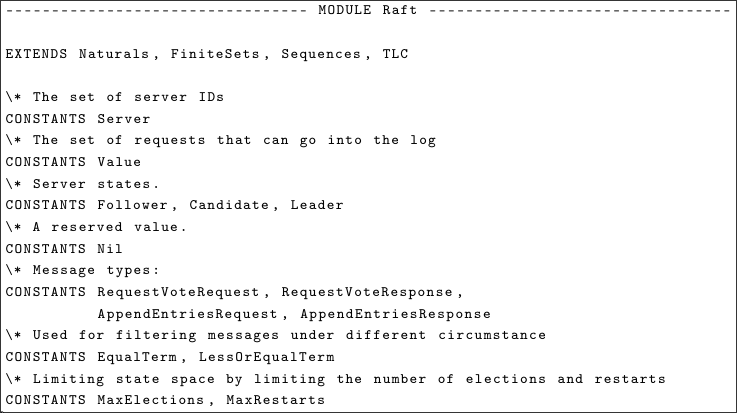
\includegraphics[scale=0.6]{inc/tla-01.png}
  \caption{Описание констант спецификации}
  \label{fig:tla-01}
\end{figure}

На рис. \ref{fig:tla-01} описана «основная среда» протокола: какие есть сервера,
значения, роли (Follower/Candidate/Leader), типы сообщений, специальные маркеры
вроде Nil и ограничения для упрощения моделирования.

$EXTENDS$ перечисляет, какие стандартные модули TLA+ были подключены:

\begin{itemize}
    \item $Naturals$: для работы с натуральными числами и базовыми операциями;
    \item $FiniteSets$: предоставляет операции над конечными множествами
        (например, $SUBSET(S)$);
    \item $Sequences$: даёт операции над последовательностями (например, $Len$,
        $Append$, $SubSeq$ и т.д.);
    \item $TLC$: вспомогательные средства моделирования (такие как $Permutations$,
        $Print$ и пр.), а также операторы типа $CHOOSE$.
\end{itemize}

$CONSTANTS$ $Server$ - множество идентификаторов серверов. Традиционно, когда
описывается система, состоящая из набора процессов/узлов, в TLA+ они задаются
как константа-множество (например, $\{s1, s2, s3\}$).

$CONSTANTS$ $Value$ – множество возможных «значений» (запросов), которые могут
добавляться в журналы (logs) серверов.

$\text{CONSTANTS Follower, Candidate, Leader}$ – три константы, обозначающие
состояния серверов в Raft: Последователь (Follower), Кандидат (Candidate)
и Лидер (Leader).

$CONSTANTS$ $Nil$ – специальное «пустое» значение. Применяется в случаях, когда
нужно указать «отсутствие чего-либо».

Блок ${CONSTANTS}$ $RequestVoteRequest$, $RequestVoteResponse$,
$AppendEntriesRequest$, $AppendEntriesResponse$ – четыре типа сообщений в Raft:
запрос на голосование, ответ на запрос голосования, запрос на добавления записей
в журнал и ответ на добавление соответственно.

$\text{CONSTANTS EqualTerm, LessOrEqualTerm}$ – два способа проверки периода (терма),
которые используются при обработке сообщений: равенство периодов (EqualTerm) или
меньшее/равное (LessOrEqualTerm).

$\text{CONSTANTS MaxElections, MaxRestarts}$ – ограничения для ограничения
пространства состояний (количество возможных выборов лидера и рестартов узлов).

\subsubsection*{Глобальные переменные}

Глобальная переменная (разделяемая между всеми серверами) только одна: $messages$.
Она представляет собой «мультимножество» сообщений, которые циркулируют в системе.
В коде это представлено как функция вида $Message \rightarrow Nat$, где $Nat$ –
сколько раз сообщение встречается (сколько копий есть в канале).

\subsubsection*{Вспомогательные переменные}

На рис. \ref{fig:tla-02} представлены вспомогательные переменные.

\begin{figure}
  \centering
  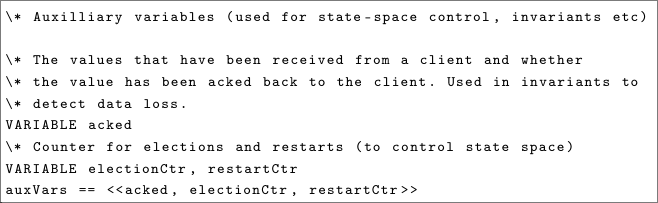
\includegraphics[scale=0.6]{inc/tla-02.png}
  \caption{Описание вспомогательных переменных}
  \label{fig:tla-02}
\end{figure}

$acked$ - это отображение вида $Value \rightarrow \{Nil, FALSE, TRUE\}$. Оно
показывает, было ли значение «подтверждено» (acked) сервером обратно клиенту.
Если $acked[v] = FALSE$, то запрос клиента уже поступил, но ещё не подтверждён;
если $TRUE$, то подтверждён. Если $Nil$, значит, это значение пока вообще не
предлагалось. Переменная используется в инвариантах для проверки отсутствия
потери данных.

$electionCtr$ и $restartCtr$ – счётчики, ограничивающие пространство состояний.
Определяют число выборов и рестартов, их максимальное значение задано константами
$MaxElections$, $MaxRestarts$, которые были описаны выше.

\subsubsection*{Переменные сервера}

Все переменные, приведенные на рис. \ref{fig:tla-03} определены для каждого
сервера. Т.е. каждая из них - функция от идентификатора сервера, задаваемого
констатами в $Server$.

\begin{figure}
  \centering
  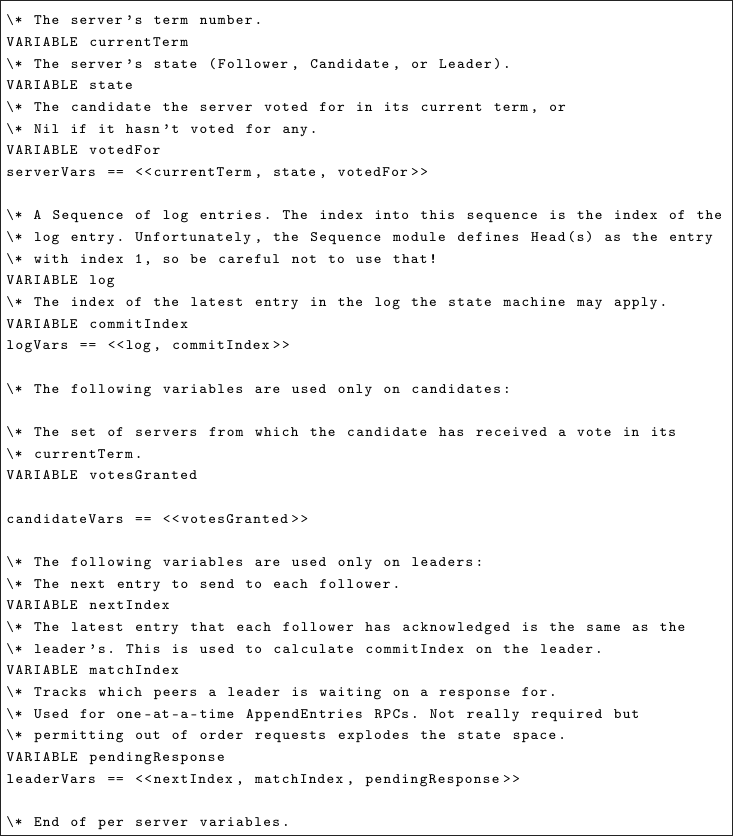
\includegraphics[scale=0.6]{inc/tla-03.png}
  \caption{Переменные сервера}
  \label{fig:tla-03}
\end{figure}

$currentTerm$ – для каждого сервера i хранит номер (терм) текущего периода Raft.
$state$ – текущее состояние сервера: $Follower$, $Candidate$ или $Leader$, как
было указано в константах.

$votedFor$ - для каждого сервера хранит, кому он отдал голос в текущем терме
(или Nil, если ещё не голосовал). Все они сгруппированы в переменную $serverVars$
для удобства обращения (например, в $WF\_vars(Next)$).

$log$ - функция от $Server$, где каждому серверу ставится в соответствие
последовательность ($Sequence$) записей в журнале. Элемент журнала обычно
содержит $(term, value)$.

$commitIndex$ показывает, до какого индекса журнал считается подтвержденнным
(т.е. готовым к применению к машине состояний).

$votesGranted$ – для сервера, который находится в состоянии $Candidate$, здесь
хранится множество серверов, которые этому кандидату дали голос в текущем терме.

$nextIndex$ – для каждого лидера и для каждого сервера в кластере хранит индекс,
с которого лидер должен отправлять записи в лог для репликации. То есть,
если $nextIndex[i][j] = k$, значит лидер $i$ собирается отправить серверу $j$ записи,
начиная с индекса $k$ (в логе самого лидера).

$matchIndex$ – для лидера $i$ и сервера $j$ указывает, до какого индекса журнала
сервер $j$ гарантированно имеет те же записи, что и лидер.

$pendingResponse$ – для лидера $i$ и сервера $j$ это булево значение, показывающее,
ждет ли лидер ответа на предыдущий RPC. Если $TRUE$, значит лидер уже отправил запрос
$AppendEntries$ серверу $j$ и ещё не получил ответа; чтобы в модели не плодилось
слишком много состояний, запрещено отправлять параллельные $AppendEntries$ одному
и тому же серверу.

\subsubsection*{Вспомогательные функции}

Реализация всех вспомогательных функций представлена на рис. \ref{fig:tla-04}.
Они не используются в инициализации системы, пересылке или обработке сообщений.

$Quorum$ – множество всех подмножеств серверов, которые образуют мажоритарный
кворум (подмножество, размер которого более половины). Если размер кластера $N$,
то в кворуме строго более $N/2$ узлов. Каждый кворум пересекается с любым другим
кворумом хотя бы в одном узле.

$LastTerm(xlog)$ – возвращает терм последней записи в журнале, или 0, если журнал
пуст.

$\_SendNoRestriction(m)$ – отправить сообщение $m$, увеличив счётчик копий в
$messages$. Если сообщение уже есть, увеличим счётчик, если нет – добавим новую
запись $m :> 1$.

\begin{figure}
  \centering
  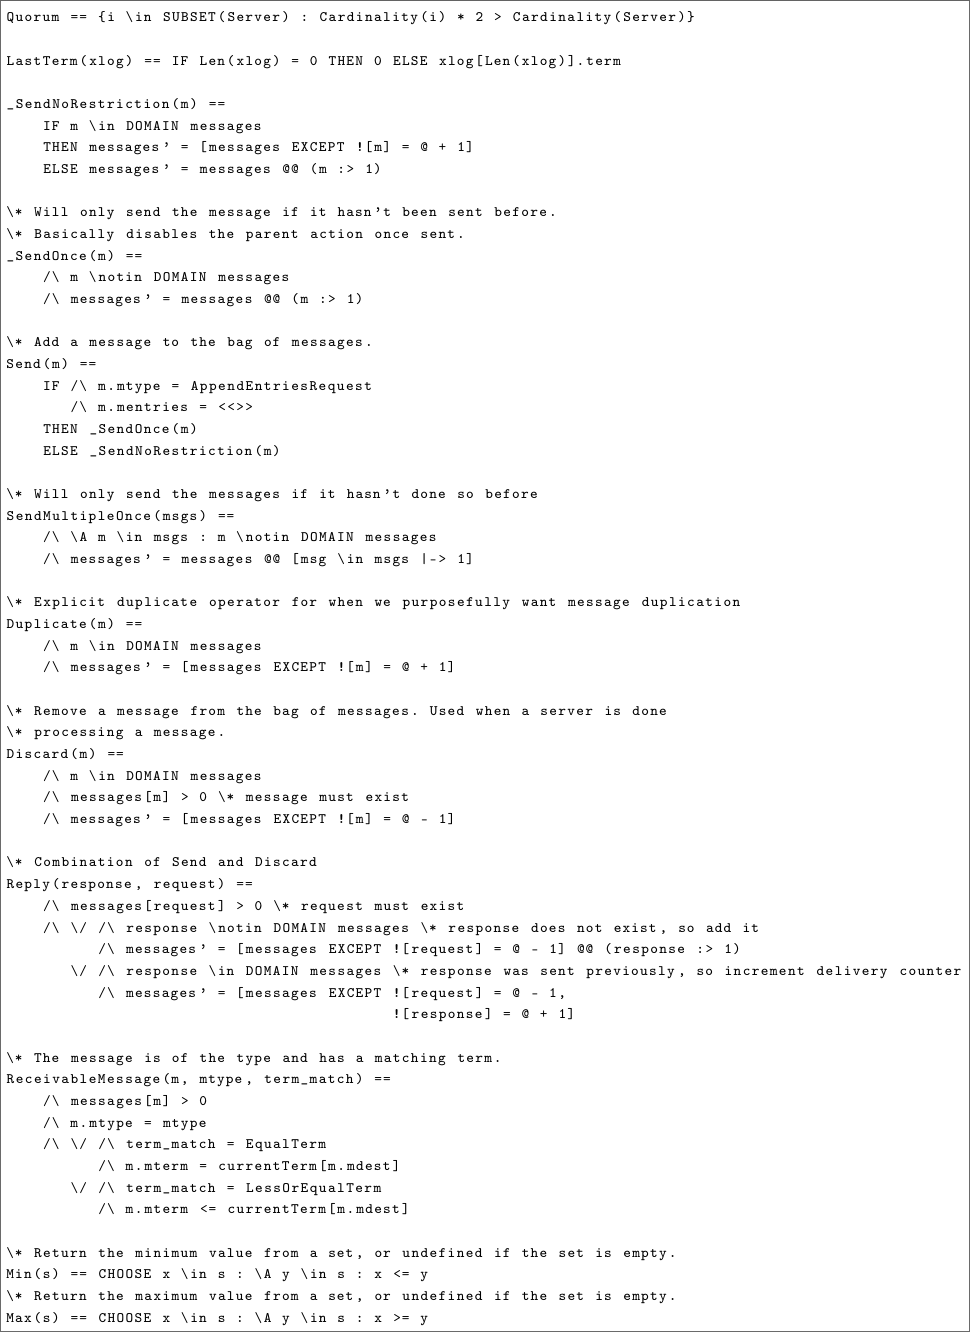
\includegraphics[scale=0.5]{inc/tla-04.png}
  \caption{Вспомогательные функции}
  \label{fig:tla-04}
\end{figure}

$\_SendOnce(m)$ – отправить сообщение m только один раз. Действие разрешено
только если такого сообщения ещё нет в $messages$. Это используется для тех
случаев, когда повторная отправка может сильно увеличивать пространство состояний
(например, пустые RPC не должны слаться бесконечно).

$Send(m)$ – оператор отправки сообщения. Если это $AppendEntriesRequest$ без
данных ($mentries=<<>>$), то используем правило «послать только один раз»; иначе
же можно добавлять в мешок сколько угодно раз.

$SendMultipleOnce(msgs)$ – отправляем сразу несколько сообщений за один шаг, но
только если ни одно из них ранее не присутствовало. Множество $msgs$ – набор
сообщений (часто это рассылка $RequestVote$ всем остальным).

$Duplicate(m)$ – искусственно дублирует сообщение, увеличивая его счётчик.
Это отдельное действие «сеть может продублировать сообщение».

$Discard(m)$ – «убрать одно вхождение сообщения из мешка». Если там несколько
копий, счётчик уменьшится на 1. Обычно вызывается после обработки сообщения
сервером.

$Reply(response, request)$ – соединяет операцию «удалить входящее сообщение
$(request)$» и «положить/увеличить ответ (response)» за один шаг. Если ответ уже
существует, увеличиваем счётчик; если нет – добавляем.

$Min/Max$ – функции для выборки минимального/максимального элемента из множества.

\subsubsection*{Инициализация}

На рис. \ref{fig:tla-05} представлена инициализация модели, по выполнении которой
формируется полное начальное состояние Raft-кластера: все сервера Follower’ы с
термом 1, без записей в журнале, без активных сообщений и с нулевыми счётчиками.

Важно отметить, что все переменные, кроме $electionCtr$, $restartCtr$, $acked$ и
$messages$ объявляются как функция от $Server$ ($\text{i in Server |->}$), можно
воспринимать их также как таблицу $map$.

\begin{figure}
  \centering
  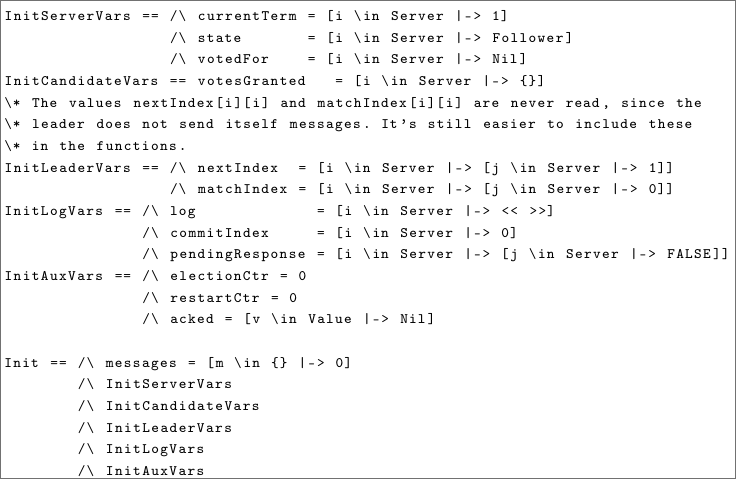
\includegraphics[scale=0.6]{inc/tla-05.png}
  \caption{Инициализация модели}
  \label{fig:tla-05}
\end{figure}

\subsubsection*{Действия}

В Raft есть несколько ключевых переходов. Каждый переход описывает, при каких
условиях он выполняется и как меняет состояние. Затем все они объединяются в
оператор $Next$, который говорит: «возможен любой из этих переходов».

\textbf{Restart}

Код метода $Restart$ представлен на рис. \ref{fig:tla-06-restart}. Он переводит
сервер в состояние $Follower$, сбрасывает все «volatile» переменные ($votesGranted$,
$nextIndex$, $matchIndex$, $pendingResponse$, $commitIndex$), увеличивает счётчик
$restartCtr$. При этом не изменяются «persistent» переменные: терм ($currentTerm[i]$),
$votedFor[i]$, сам журнал ($log[i]$), уже подтверждённые значения. Условие
$restartCtr < MaxRestarts$ ограничивает количество рестартов.

\begin{figure}
  \centering
  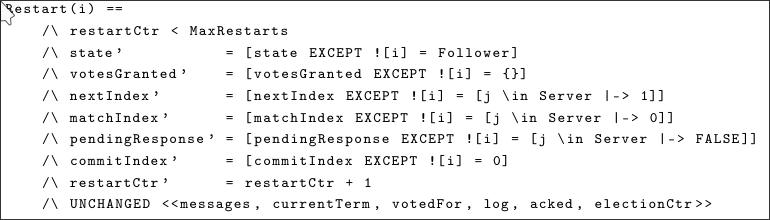
\includegraphics[scale=0.4]{inc/tla-06-restart.png}
  \caption{Метод $Restart$}
  \label{fig:tla-06-restart}
\end{figure}

\textbf{RequestVote}

Код метода $RequestVote$ представлен на рис. \ref{fig:tla-06-request-vote}. Сервер
$i$ будучи в состоянии $Follower$ или $Candidate$, начинает новые выборы следующим
образом:

\begin{enumerate}
    \item Проверка, что ещё не превышен $MaxElections$;
    \item Состояние меняется в $Candidate$;
    \item Терм увеличивается на 1;
    \item Отдается голос самому себе: $votedFor[i] = i$;
    \item Увеличивается счетчик выборов;
    \item Рассылаются запросы на голос всем серверам, кроме себя ($RequestVoteRequest$).
\end{enumerate}

\begin{figure}
  \centering
  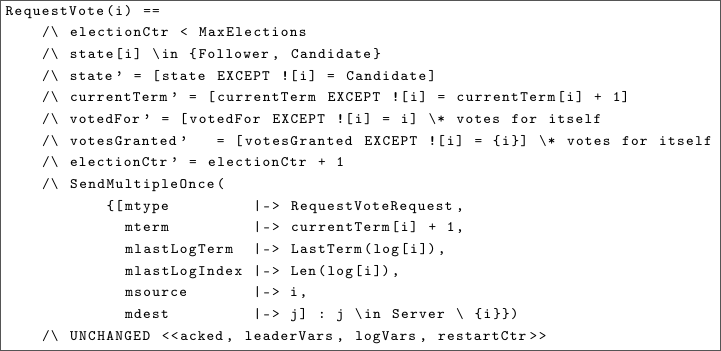
\includegraphics[scale=0.4]{inc/tla-06-request-vote.png}
  \caption{Метод $RequestVote$}
  \label{fig:tla-06-request-vote}
\end{figure}

\textbf{AppendEntries}

Код метода $AppendEntries$ представлен на рис. \ref{fig:tla-06-append-entries}.

\begin{figure}
  \centering
  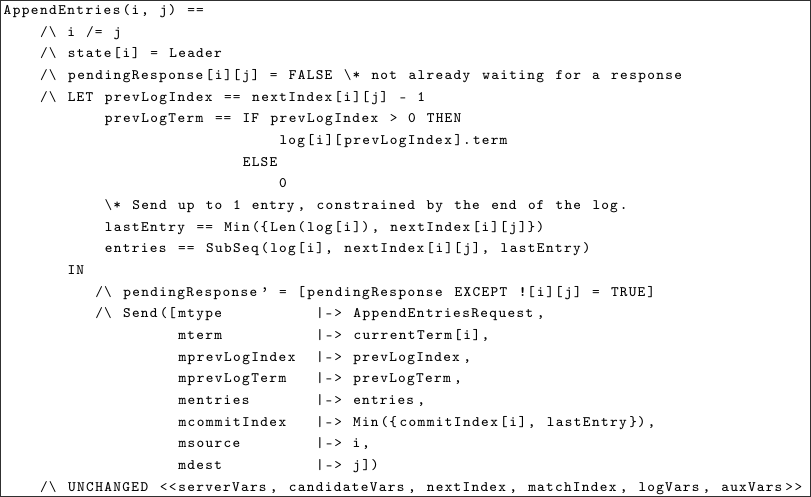
\includegraphics[scale=0.4]{inc/tla-06-append-entries.png}
  \caption{Метод $AppendEntries$}
  \label{fig:tla-06-append-entries}
\end{figure}

Лидер $i$ отправляет запрос $AppendEntriesRequest$ последователю $j$. В сообщении
не может быть больше одной записи $entry$. Условие $\text{pendingResponse[i][j] = FALSE}$
гарантирует, что не отправляем новый RPC, пока старый еще без ответа.

\textbf{BecomeLeader}

Код метода $BecomeLeader$ представлен на рис. \ref{fig:tla-06-become-leader}.
Сервер-кандидат $i$ обнаруживает, что у него есть кворум голосов (в $votesGranted[i]$).
Значит, он выигрывает выборы и становится лидером. Переводится $state[i]$ в $Leader$,
инициализируется $nextIndex[i]$, $matchIndex[i]$, $pendingResponse[i]$. Другие
переменные не меняются.

\begin{figure}
  \centering
  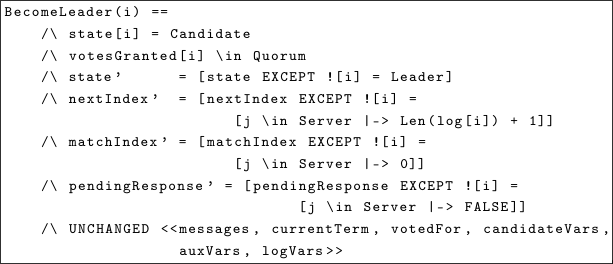
\includegraphics[scale=0.4]{inc/tla-06-become-leader.png}
  \caption{Метод $BecomeLeader$}
  \label{fig:tla-06-become-leader}
\end{figure}

\textbf{AdvanceCommitIndex}

Код метода $AdvanceCommitIndex$ представлен на рис. \ref{fig:tla-06-advance-commit-index}.

\begin{figure}
  \centering
  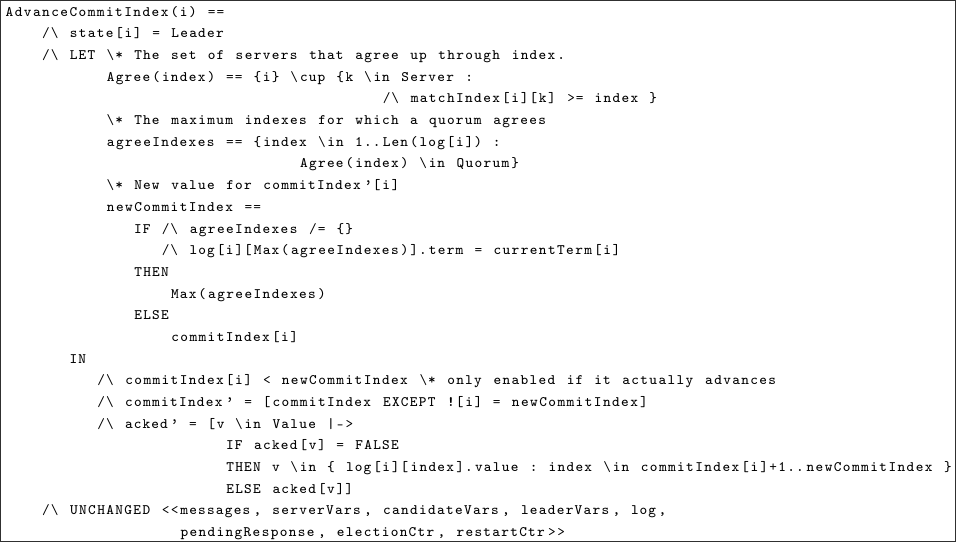
\includegraphics[scale=0.4]{inc/tla-06-advance-commit-index.png}
  \caption{Метод $AdvanceCommitIndex$}
  \label{fig:tla-06-advance-commit-index}
\end{figure}

Лидер $i$ пытается продвинуть свой $commitIndex$ вперёд, если есть подтверждение
большинства узлов для определённого индекса. Для этого проверяется множество
серверов, у которых $matchIndex[i][k] >= index$, и вычисляется максимум индексов,
по которым у лидера есть кворум. Если этот индекс принадлежит текущему терму лидера,
обновляется $commitIndex[i]$. Все значения, которые таким образом становятся
закоммиченными, теперь помечаются $acked[v] = TRUE$.

\textbf{UpdateTerm}

Код метода $UpdateTerm$ представлен на рис. \ref{fig:tla-06-update-term}.
Если где-то в сети есть сообщение с термом больше, чем у сервера, который
его получит, то сервер «обновляет» свой терм, сбрасывает своё голосование,
становится $Follower$.

\begin{figure}
  \centering
  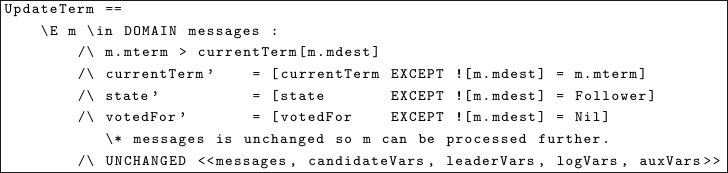
\includegraphics[scale=0.4]{inc/tla-06-update-term.png}
  \caption{Метод $UpdateTerm$}
  \label{fig:tla-06-update-term}
\end{figure}

\textbf{HandleRequestVoteRequest}

Код метода $HandleRequestVoteRequest$ представлен на рис. \ref{fig:tla-06-handle-request-vote}.

\begin{figure}
  \centering
  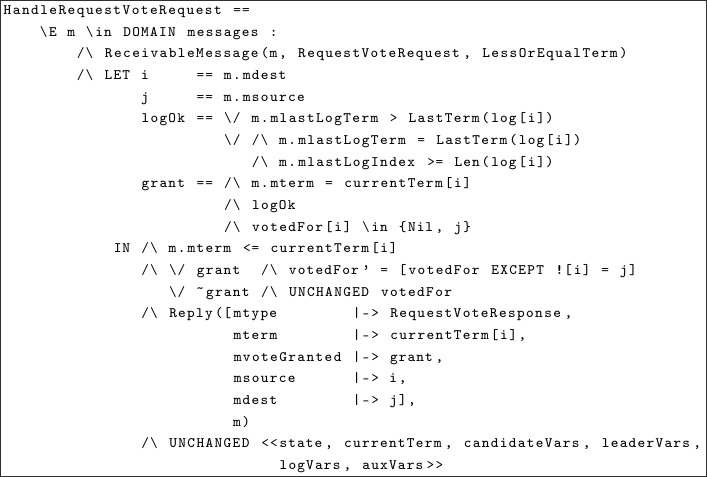
\includegraphics[scale=0.4]{inc/tla-06-handle-request-vote.png}
  \caption{Метод $HandleRequestVoteRequest$}
  \label{fig:tla-06-handle-request-vote}
\end{figure}

Сервер $i$ обрабатывает входящий $RequestVoteRequest$ от сервера $j$. Сначала
проверяется условие $\textit{ReceivableMessage(..., LessOrEqualTerm)}$, то есть
терм запроса не больше текущего, иначе этим занялось бы $UpdateTerm$. Затем
проверяется «лог последнего кандидата»: \textit{(m.mlastLogTerm, m.mlastLogIndex)}
сравнивается с собственным журналом. Если лог кандидата не меньше нашего, и сам
сервер $i$ ещё не голосовал в этом терме (или уже голосовал за $j$), мы отдадим
ему голос. Результат — отправка $RequestVoteResponse$ с $mvoteGranted = grant$.

\textbf{HandleRequestVoteResponse}

Код метода $HandleRequestVoteResponse$ представлен на рис.
\ref{fig:tla-06-handle-request-vote-response}. Сервер $i$ получает ответ на
запрос голосования от $j$. Если $mvoteGranted = TRUE$, добавляем $j$ в
$votesGranted[i]$. Иначе ничего не делаем. Сообщение удаляется из сети после
обработки.

\begin{figure}
  \centering
  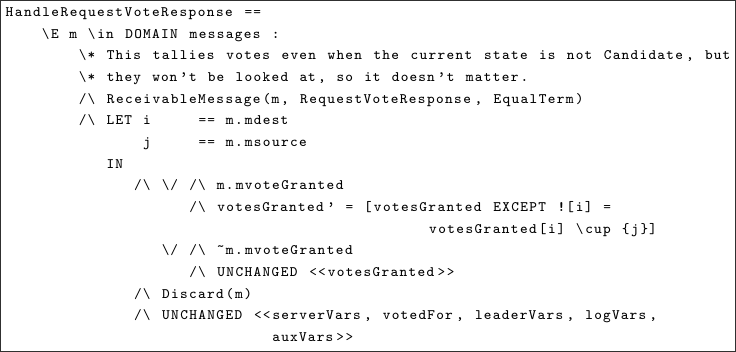
\includegraphics[scale=0.4]{inc/tla-06-handle-request-vote-response.png}
  \caption{Метод $HandleRequestVoteResponse$}
  \label{fig:tla-06-handle-request-vote-response}
\end{figure}

\textbf{RejectAppendEntriesRequest}

Код метода $RejectAppendEntriesRequest$ представлен на рис.
\ref{fig:tla-06-reject-append-entries}.
Сервер $i$ отвергает $AppendEntriesRequest$, если терм сообщения меньше его
собственного либо если термы равны, но у получателя – $Follower$, и при этом
журнал «не совпадает» (поле $m.mprevLogTerm$ или $m.mprevLogIndex$ не
соответствуют локальному журналу).

\begin{figure}
  \centering
  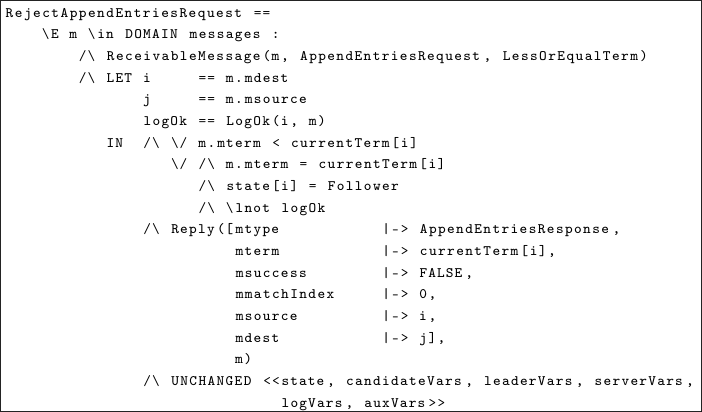
\includegraphics[scale=0.4]{inc/tla-06-reject-append-entries.png}
  \caption{Метод $RejectAppendEntriesRequest$}
  \label{fig:tla-06-reject-append-entries}
\end{figure}

В ответ отправляется $AppendEntriesResponse$ с $msuccess = FALSE$.

\textbf{AcceptAppendEntriesRequest}

Код метода $AcceptAppendEntriesRequest$ представлен на рис.
\ref{fig:tla-06-accept-append-entries}.
Может произойти урезание лога и/или добавление одной записи. $commitIndex'[i]$
устанавливается равным тому, что лидер прислал в $m.mcommitIndex$, так как
$Follower$ следует за лидером. Отправляем положительный ответ ($AppendEntriesResponse$)
с $msuccess = TRUE$.

\begin{figure}
  \centering
  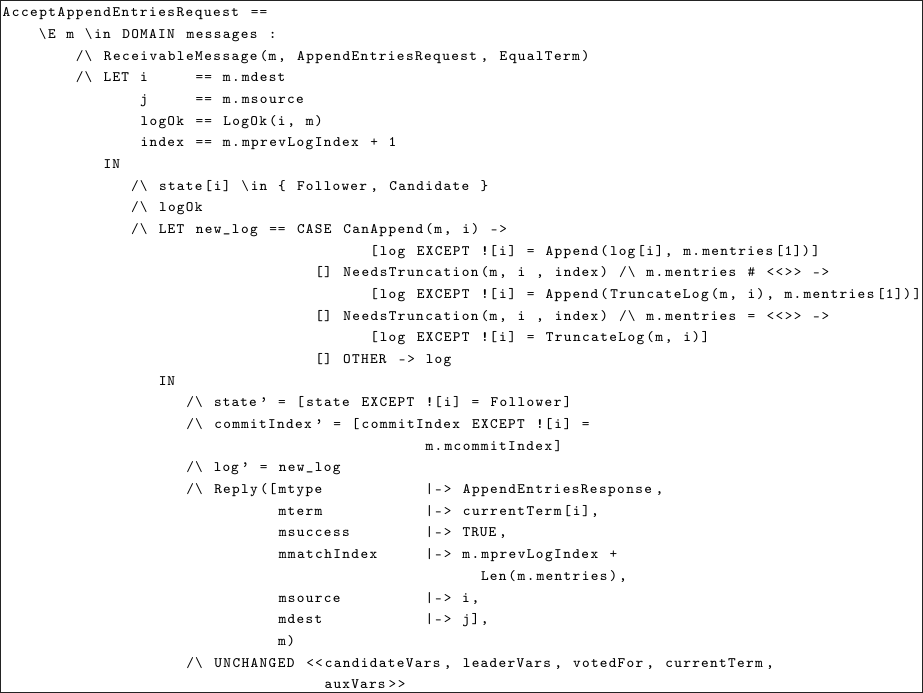
\includegraphics[scale=0.4]{inc/tla-06-accept-append-entries.png}
  \caption{Метод $AcceptAppendEntriesRequest$}
  \label{fig:tla-06-accept-append-entries}
\end{figure}

\textbf{HandleAppendEntriesResponse}

Код метода $HandleAppendEntriesResponse$ представлен на рис.
\ref{fig:tla-06-handle-accept-append-entries-response}.

\begin{figure}
  \centering
  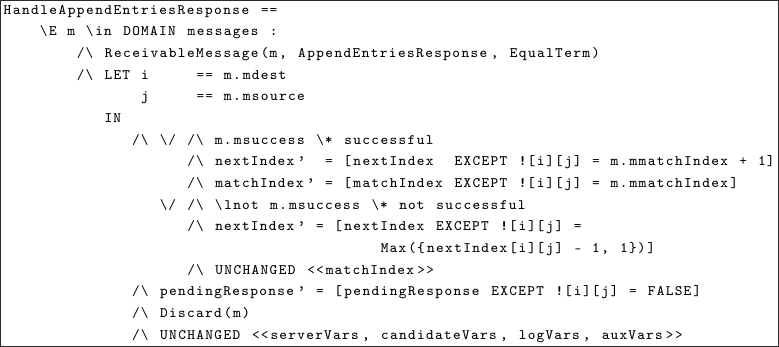
\includegraphics[scale=0.4]{inc/tla-06-handle-append-entries-response.png}
  \caption{Метод $HandleAppendEntriesResponse$}
  \label{fig:tla-06-handle-append-entries-response}
\end{figure}

Лидер $i$ получает ответ от $j$. Если $m.msuccess = TRUE$, значит $j$ у себя
добавил записи, и лидер ставит $matchIndex[i][j] = mmatchIndex$. $nextIndex[i][j]$
становится $mmatchIndex + 1$. Если $FALSE$, значит у $j$ оказались расхождения,
и тогда лидер уменьшает $nextIndex[i][j]$ на 1, чтобы попробовать снова.
$pendingResponse'[i][j] = FALSE$ – освобождается «окно» для следующего запроса.
Затем сообщение выбрасывается из сети.

\subsubsection*{Спецификация и оператор Next}

Код оператора и спецификации приведен на рис. \ref{fig:tla-07}

\begin{figure}
  \centering
  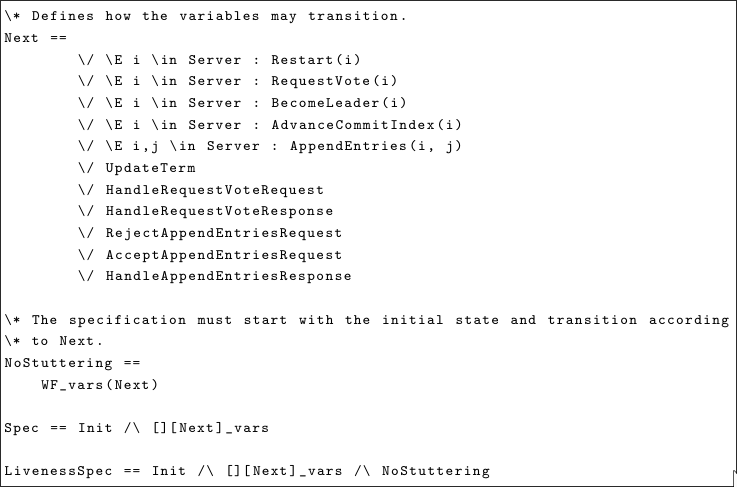
\includegraphics[scale=0.4]{inc/tla-07.png}
  \caption{Спецификация и оператор $Next$}
  \label{fig:tla-07}
\end{figure}

Оператор $Next$ представляет собой главную дизъюнкцию всех возможных действий,
которые могут происходить в любой момент. Система в каждый момент времени может
сделать один из перечисленных переходов (\textit{Restart, RequestVote, AppendEntries,
BecomeLeader} и т.п.), если выполняются условия.

$Spec$ – классическая структура TLA+ спецификации: $Init$ задаёт начальное
состояние, $[][Next]\_vars$ говорит, что на каждом шаге выполняется одно из
действий $Next$.

\subsubsection*{Инварианты}

Инварианты представлены на рис. \ref{fig:tla-08}. Они проверяются моделью, описанной
в следующей части, чтобы убедиться, что Raft-свойства не нарушаются при любых
последовательностях действий.

\begin{figure}
  \centering
  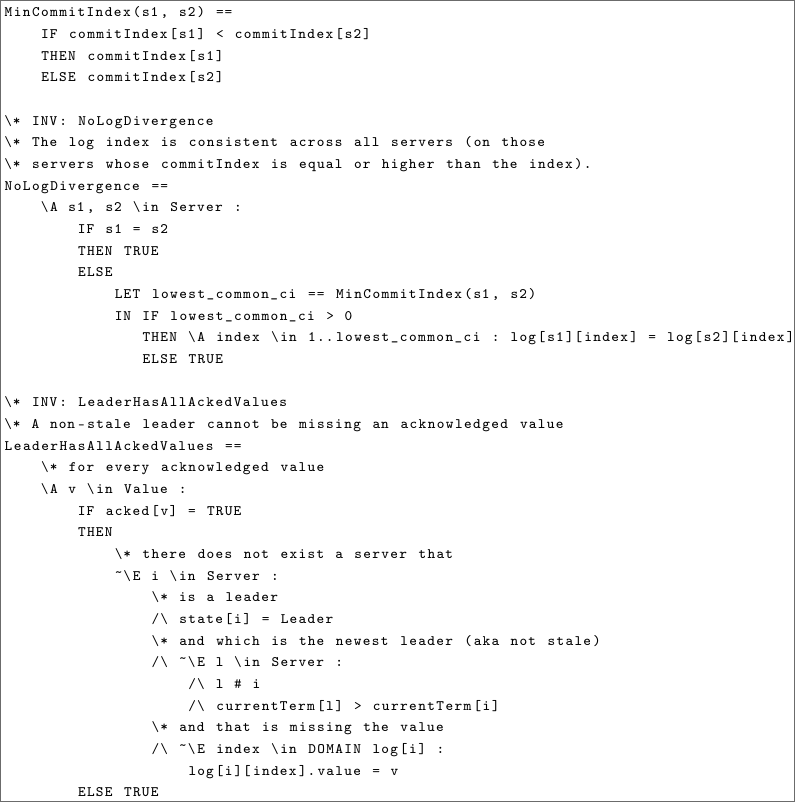
\includegraphics[scale=0.4]{inc/tla-08.png}
  \caption{Инварианты}
  \label{fig:tla-08}
\end{figure}

$NoLogDivergence$ – инвариант о том, что если у двух серверов некий индекс
подтвержден (меньшее из их commitIndex), то записи по этому индексу совпадают.
Это ключевое свойство согласованности в Raft.

$LeaderHasAllAckedValues$ – если значение ($v$) уже подтверждено как
$acked[v] = TRUE$, то любой лидер обязан иметь это значение в своём логе.

\subsubsection*{Итого}

Данная спецификация описывает основные аспекты Raft:

\begin{enumerate}
    \item Состояния узлов (\textit{Follower, Candidate, Leader}) и их персистентные
        переменные (\textit{currentTerm, votedFor, log}).
    \item Обмен сообщениями (\textit{RequestVote, AppendEntries} и их ответы) через
        переменную $messages$.
    \item Логика перехода (кандидат пытается стать лидером, лидер реплицирует
        записи, узлы отвечают и обновляют термы, если видят более высокий терм,
        и т.д.).
    \item Инварианты (\textit{NoLogDivergence, LeaderHasAllAckedValues}, и пр.),
        которые отражают ключевые свойства безопасности Raft.
\end{enumerate}

Таким образом, в модели учтены основные механизмы Raft: выбор лидера, поддержка
согласованного журнала, коммиты и гарантии о том, что система не теряет
записанные и закоммиченные данные.

\subsection{Проверка модели}

В TLA+ модель проверяется с помощью TLC, перебирающего всевозможные (или
ограниченные) пути выполнения спецификации и проверяющего инварианты.

В приложении Б приведен код конфигурации модели для TLC, в котором задаются
значения констант, какие варианты проврять, какой оператор считать стартовым и
переходным.

Результаты проверки приведены на рис. \ref{fig:tla-09}. Было проверено более 36
тысяч возможных состояний, инварианты не нарушаются.

\begin{figure}
  \centering
  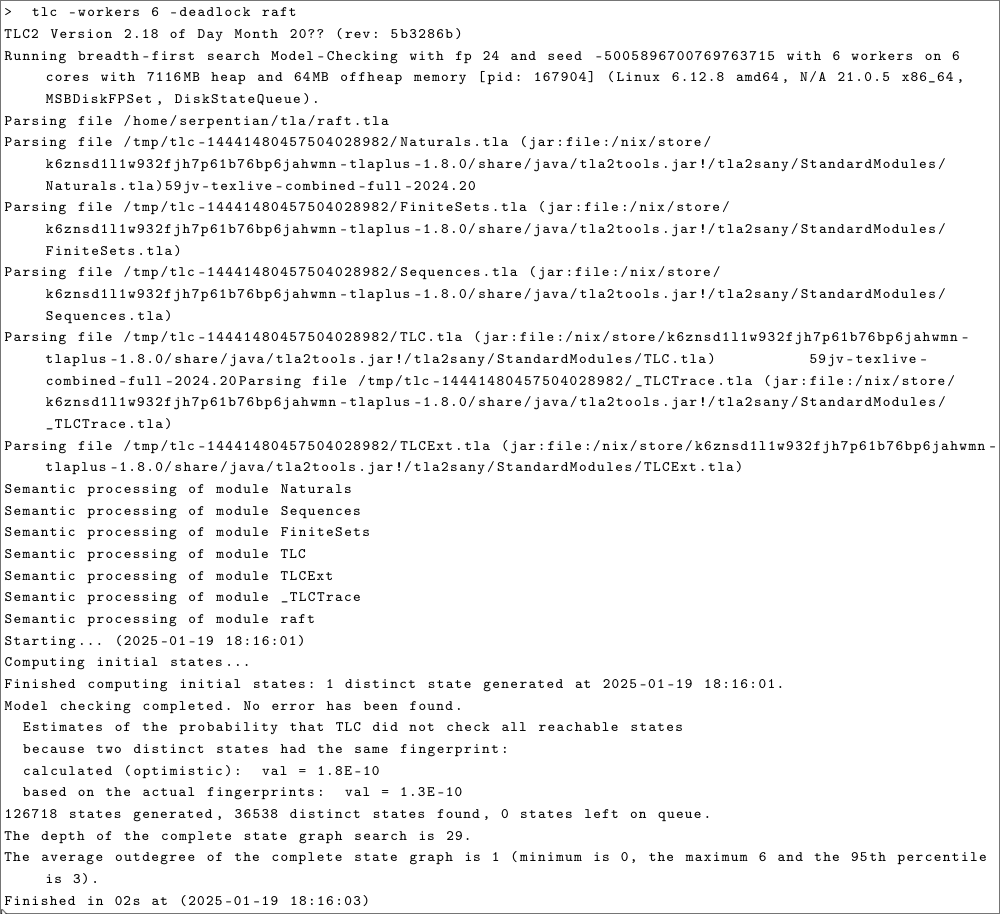
\includegraphics[scale=0.4]{inc/tla-09.png}
  \caption{Проверка модели}
  \label{fig:tla-09}
\end{figure}


    \conclusion

В ходе прохождения практики был проведён комплексный анализ механизма
шардирования в СУБД Tarantool. Основное внимание было уделено изучению
архитектуры модуля \texttt{vshard}, принципов распределения данных и
обеспечения согласованности при выполнении операций в шардированном кластере.

Были рассмотрены и проанализированы существующие подходы к реализации
Map-Reduce запросов по репликам. В результате исследования выявлены ключевые
проблемы, связанные с обеспечением консистентности данных при выполнении
распределённых запросов, и предложена альтернативная реализация.

Практическая значимость работы заключается в:
\begin{itemize}
    \item Систематизации знаний о работе шардированного кластера Tarantool;
    \item Выявлении ограничений существующей реализации модуля \texttt{vshard};
    \item Разработке предложений по расширению функциональности для поддержки
        Map-Reduce операций по репликам.
\end{itemize}

Полученные результаты могут быть использованы для дальнейшего развития модуля
шардирования Tarantool и улучшения его безопасности. Проведённое исследование
демонстрирует важность комплексного подхода к проектированию распределённых
систем и необходимость тщательного анализа требований к согласованности данных.

Результаты работы подтверждают возможность реализации эффективного механизма
выполнения Map-Reduce запросов по репликам в шардированной среде с соблюдением
требований к консистентности данных и производительности системы.


    \printbibliography

    \appendix
    \appendixsection{Основы теории решёток}

В последние годы решётки служат алгоритмическим инструментом для решения
широкого круга задач в информатике, математике и криптографии, особенно в
квантовоустойчивых криптографических протоколах. Ниже приведены базовые понятия
и известные алгоритмы, тесно связанные с нашей работой.

\subsection*{Базовые понятия}

Пусть $\lVert\cdot\rVert$ — евклидова норма векторов из $R^{m}$. Векторы
отмечаем полужирным (в переводе этого нет), матрицы пишем построчно; элементы
матрицы $M$ обозначаем $m_{i,j}$. Верхний индекс~$T$ — транспонирование.

\begin{itemize}
\item \textbf{Решётка.} Пусть $b_{1},\ldots,b_{n}\in R^{m}$ — линейно
        независимые столбцы, тогда множество всех линейных комбинаций их
        целочисленных коэффициентов — решётка, определяемая как
        \begin{equation} \Lambda(B) =\{\,Bx \mid x\in Z^{n}\,\} =\{\,b =
            x_{1}b_{1}+\dots+x_{n}b_{n} \mid x_{1},\dots,x_{n}\in Z\,\}.
        \end{equation} где $B=[b_{1},\ldots,b_{n}]\in R^{m\times n}$ — матрица
        базиса, которая также может быть использована чтобы представлять
        решетку для простоты. $\{b_1, \ldots, b_n\}$ - группа базиса решетки.
        Размерность решётки $n$. Её детерминант $\det\Lambda=(\det
        B^{T}B)^{1/2}$, здесь $B^T$ - транспонированная матрица $B$. При
        квадратной $B$ имеем $\det\Lambda=\det B$. Детерминант представляет
        объём решётки в геометрическом представлении, обозначается как
        $\operatorname{vol}(\Lambda)$. Длина точки $b\in R^{m}$ определяется
        как $\lVert b\rVert=(b^{T}b)^{1/2}$.

\item \textbf{Последовательные минимумы.} Для $n$‑мерной решётки $\Lambda$
        положительные числа $\lambda_{1}(\Lambda)\le\lambda_{2}(\Lambda)
        \le\dots\le\lambda_{n}(\Lambda)$ называются последовательными
        минимумами, где $\lambda_{k}(\Lambda)$ — наименьший радиус шара с
        центром в нуле, содержащего $k$ линейно независимых векторов из
        $\Lambda$. Обозначим $\lambda_{1}=\lambda_{1}(\Lambda)$ как длину
        кратчайшего ненулевого вектора из $\Lambda$.

\item \textbf{Постоянная Эрмита.} Эрмитовым инвариантом решётки $\Lambda$
        называется
        \begin{equation}
          \gamma(\Lambda)
          = \frac{\lambda_{1}^{2}(\Lambda)}{\operatorname{vol}(\Lambda)^{2/n}}
          = \frac{\lambda_{1}^{2}(\Lambda)}{\det(\Lambda)^{2/n}}.
        \end{equation}

        Постоянная Эрмита $\gamma_{n}$ — максимальное значение $\gamma(\Lambda)$
        для всех $n$‑мерных решёток, или минимальное константное $\gamma$,
        удовлетворяющее $\lambda_{1}(\Lambda)^{2}\le\gamma(\det\Lambda)^{2/n}$
        для всех решёток размености $n$ соответственно.

\item \textbf{QR‑разложение.} У решёточной матрицы базиса $B$ есть единственное
        разложение $B=QR\in R^{m\times n}$, где $Q\in R^{m\times n}$,
        $R=[r_{i,j}]_{1\le i,j\le n} \in R^{n\times n}$, здесь $Q\in R^{m\times
        n}$ — изомет­рическая (столбцы ортогональны и единичной длины), а $R
        \in R^{n\times n}$ — верхнетреугольная матрица с положительными
        диагональными элементами $r_{i,i}$. Коэффициенты Грама–Шмидта
        $\mu_{j,i}=r_{i,j}/r_{i,i}$ легко вычисляются из QR‑разложения. Для
        целочисленной $B$ коэффициенты $\mu_{j,i}$ обычно рациональны.

\item \textbf{Задача кратчайшего вектора (SVP).}
      Дана группа базиса $B$ решётки $\Lambda$.

      \begin{itemize}
          \item Задача кратчайшего вектора (SVP): Требуется найти вектор
              $v\in\Lambda$, такой что $\lVert v\rVert=\lambda_{1}(\Lambda)$.
          \item Приближённая задача кратчайшего вектора ($\alpha$‑SVP): Найти
              ненулевой вектор $v\in\Lambda$, удовлетворяющий
              $\lVert v\rVert\le\alpha\,\lambda_{1}(\Lambda)$.
          \item Эрмитова задача кратчайшего вектора ($r$‑Hermite SVP):
              Найти ненулевой вектор $v\in\Lambda$, такой что
              $\lVert v\rVert \;\le\; r\,\det(\Lambda)^{1/n}$.
      \end{itemize}

      Параметр $\alpha\ge1$ в $\alpha$‑SVP называется фактором аппроксимации.
      Обычнро задача упрощается при увеличении $\alpha$. При $\alpha=1$ задачи
      $\alpha$‑SVP и SVP совпадают. Истинное значение $\lambda_{1}$ в
      $\alpha$‑SVP трудно вычислить из-за сложности SVP, поэтому решение
      $\alpha$‑SVP не всегда легко проверить. Задача $r$‑Hermite SVP является
      вычислимой (относительно просто вычислимой), она определяется величиной
      $\det(\Lambda)^{1/n}$ вместо $\Lambda_1$. В результате, мы можем лешко
      проверить решение, но не можем сравнить его с кратчайшим вектором.

\item \textbf{Задача ближайшего вектора (CVP)}
      Дана группа базиса $B$ решётки $\Lambda$ и целевой вектор
      $t\in\operatorname{span}(B)$.

      \begin{itemize}
          \item Задача ближайшего вектора (CVP): Найти вектор $v\in\Lambda$,
              такой что расстояние $\lVert v - t\rVert$ может быть минимизировано,
              т.е. $\lVert v - t\rVert = \operatorname{dist}(\Lambda,t)$.
          \item $\alpha$-приближенная задача ближайшего вектора ($\alpha$‑CVP):
              Найти вектор $v\in\Lambda$, такой что расстояние
              $\lVert v - t\rVert \le \alpha \times \operatorname{dist}(\Lambda,t)$
          \item $r$-приближенная задача ближайшего вектора (($r$‑AbsCVP):  Найти
              $v\in\Lambda$ такое, что $\lVert v - t\rVert \le r$.
      \end{itemize}

      Определения аналогичны случаям для SVP; параметр $\alpha\ge1$ в
      $\alpha$‑CVP играет ту же роль, что и в $\alpha$‑SVP. В $r$‑AbsCVP
      параметр $r$ может быть любым разумным значением, соизмеримым с
      $\operatorname{dist}(\Lambda,t)$, например $\det(\Lambda)^{1/n}$ в
      $r$‑Hermite SVP.
\end{itemize}

\subsection*{Алгоритм LLL}
\begin{algorithm}[htp!]
    \SetAlgoLined

    \KwData{базис решётки $\text{b}_1, \dots, \text{b}_n \in \text{Z}^m$, параметр $\delta$}
    \KwResult{$\delta$-LLL-редуцированный базис}

    \textbf{Шаг 1:} Орторгонализация Грама-Шмидта \\
    Выполнить орторгонализацию Грама-Шмидта для базиса $\text{b}_1, \dots, \text{b}_n$, обозначим результат как $\tilde{\text{b}}_1, \dots, \tilde{\text{b}}_n \in \text{R}^m$

    \textbf{Шаг 2:} Редукция

    \For{$i = 2$; $i < n$; $i = i + 1$}{
        \For{$j = i-1$; $i > 1$; $ i = i - 1$}{
            $c_{i,j} = \left\lfloor \dfrac{\langle \text{b}_i, \tilde{\text{b}}_j \rangle}{\langle \tilde{\text{b}}_j, \tilde{\text{b}}_j \rangle} \right\rceil$; \\
            $\text{b}_i \gets \text{b}_i - c_{i,j} \cdot \text{b}_j$;
        }
    }

    \textbf{Шаг 3:} Обмен

    \If{$\exists \, i$ такое, что $\delta \cdot \| \tilde{\text{b}}_i \|^2 > \| \mu_{i+1,i} \tilde{\text{b}}_i + \tilde{\text{b}}_{i+1} \|^2$}{
        $\text{b}_i \leftrightarrow \text{b}_{i+1}$; \\
        перейти к шагу 1;
    }

    \textbf{Шаг 4:} Вывод базиса $\text{b}_1, \dots, \text{b}_n$

    \caption{Алгоритм LLL-редукции}
    \label{alg:lll}
\end{algorithm}

Алгоритм LLL — один из самых известных алгоритмов редукции решётки; он был
предложен А. К. Ленстрой, Х. В. Ленстрой (мл.) и Л. Ловашем в 1982 г.
\cite{cite_35}. Для $n$‑мерной решётки этот алгоритм позволяет решать $\alpha
\;=\; \left(\frac{2}{\sqrt{3}}\right)^{n}$ за полиномиальное время. Ниже
приведены связанные понятия и алгоритмы.

\newcounter{tmp-enum-lll}

\begin{itemize}
    \item \textbf{LLL базиc}: Базис $B = QR$ называется LLL‑редукции или
        LLL‑базисом при параметре редукции $\delta\in(1/4,1]$, если выполняются
        условия:
        \begin{enumerate}
            \item $\frac{\lvert r_{i,j}\rvert}{r_{i,i}} \;\le\; \frac12, \quad \text{for all } j > i;$
            \item $\delta\, r_{i,i}^{2}\;\le\;r_{i,i+1}^{2} + r_{i+1,i+1}^{2},\quad \text{for } i = 1,\ldots,n-1.$
            \setcounter{tmp-enum-lll}{\value{enumi}}
        \end{enumerate}

        Очевидно, LLL‑базис также удовлетворяет
        \( r_{i,i}^{2} \le \alpha\, r_{i+1,i+1}^{2} \),
        для \(\alpha = \frac{1}{(\delta - 1 / 4)}\).

        Параметры, рассматриваемые в оригинальной литературе по алгоритму LLL,
        равны $\delta = \tfrac34$, $\alpha = 2$. Известный результат о LLL‑базисе
        показывает, что для любого $\delta < 1$ LLL‑базис может быть получен за
        полиномиальное время и хорошо аппроксимирует последовательные минимумы\:

        \begin{enumerate}
            \setcounter{enumi}{\value{tmp-enum-lll}}
            \item $\alpha^{-\,i+1} \;\le\; \lVert b_{i}\rVert^{2}\,\lambda_{i}^{-2}
                \;\le\; \alpha^{\,n-1}, \quad \text{for } i = 1,\ldots,n;$
            \item $\lVert b_{1}\rVert^{2} \;\le\; \alpha^{\frac{n-1}{2}}\,
                \bigl(\det\Lambda\bigr)^{2/n}.$
        \end{enumerate}

    \item \textbf{Алгоритм LLL}: Для заданного набора базиса
        $B = [b_{1},\ldots,b_{n}] \in Z^{m\times n}$
        алгоритм может привести его к LLL‑редуцированному виду
        или преобразовать в LLL‑базис. Алгоритм состоит из трёх
        основных шагов: ортогонализация Грама–Шмидта, редукции и
        обмен. Конкретные шаги приведены в Алгоритме \ref{alg:lll}.
\end{itemize}

\subsection*{Алгоритм ближайшей плоскости Бабая}

Алгоритм ближайшей плоскости Бабая \cite{cite_32} (далее — алгоритм Бабая)
применяется для решения CVP. Для $n$‑мерной решётки он может получать фактор
аппроксимации $\alpha \;=\; 2\!\left(\frac{2}{\sqrt{3}}\right)^{n}$ для
$\alpha$‑CVP. Алгоритм состоит из двух этапов, первый из которых заключается в
редукции решетки с помощью алгоритма LLL. Второй является процедурой уменьшения
размера, который в основном вычисляет линейную комбинацию целочисленных
коэффициентов, ближайших к целевому вектору $t$ в LLL-базисе. Этот шаг по сути
совпадает со вторым шагом в LLL-редукции. Подробные действия приведены в
Алгоритме \ref{alg:babai}.

\begin{algorithm}[htp!]
    \SetAlgoLined

    \KwData{базис решётки $\text{b}_1, \dots, \text{b}_n \in \text{Z}^m$, параметр $\delta = 3/4$, целевой вектор $\text{t} \in \text{Z}^m$}
    \KwResult{вектор $\text{x} \in \Lambda(B)$, такой что $\|\text{x} - \text{t}\| \leq 2^{n/2} \, \text{dist}(\text{t}, \Lambda(B))$}

    \textbf{Шаг 1:} LLL-редукция \\
    Применить LLL-редукцию к базису $B$ с параметром $\delta$ \\
    Обозначим результат: $\tilde{\text{b}}_1, \dots, \tilde{\text{b}}_n \in \text{R}^m$

    \textbf{Шаг 2:} Уменьшение размера \\
    $\text{b} \gets \text{t}$

    \For{$j = n$; $j > 1$ $j = j-1$}{
        $c_j = \left\lfloor \dfrac{\langle \text{b}, \tilde{\text{b}}_j \rangle}{\langle \tilde{\text{b}}_j, \tilde{\text{b}}_j \rangle} \right\rceil$ \\
        $\text{b} \gets \text{b} - c_j \cdot \text{b}_j$
    }

    \textbf{Шаг 3:} Вернуть $\text{t} - \text{b}$

    \caption{Алгоритм Бабая}
    \label{alg:babai}
\end{algorithm}

    \appendixsection{Алгоритм Шнорра для факторизации целых чисел}

\subsection*{Метод решета Шнорра}

Рассмотрим общую задачу факторизации, в которой задано целое число $N$,
предполагается разложить его на два нетривиальных множителя $p<q$, так что $N =
p\times q$. Метод решета для факторизации начинается с определения пары гладких
отношений.

Пусть $p_i,\; i = 1,\dots,n$ — первые $n$ простых чисел вместе с $p_0$,
удовлетворяющими $-1 = p_0 < 1 < p_1 < \dots < p_n < p$. Множество $P =
\{p_i\}_{i=0,\dots,n}$ называется простым базисом. Число $p_0 = -1$ не является
простым, однако включается для учёта знака целого числа. Целое число называется
$p_n$‑гладким, если все его простые делители меньше $p_n$; число $p_n$ при этом
называют пределом гладкости. Пара целых чисел $(u_j,v_j)$ называется
$p_n$‑гладкой парой, если и $u_j$, и $v_j$ являются $p_n$‑гладкими. Более того,
пара целых чисел $(u_j,v_j)$ называется $p_n$‑гладкой парой отношений
(сокращённо sr‑пара), если:

\begin{equation}
  u_{j} \;=\; \prod_{i=1}^{n} p_{i}^{\,e_{i,j}},
  \qquad
  u_{j} - v_{j}N \;=\; \prod_{i=0}^{n} p_{i}^{\,e'_{i,j}},
\end{equation}

\noindent где $e_{i,j},\,e'_{i,j}\in{N}$, тогда имеем

\begin{equation}
  \frac{u_{j}-v_{j}N}{u_{j}}
  \;\equiv\;
  \prod_{i=0}^{n} p_{i}^{\,e'_{i,j}-e_{i,j}}
  \;\equiv\; 1 \pmod{N}.
\end{equation}

Следует отметить, что гладкая пара отличается от sr‑пары: sr‑пара должна не
только быть $p_n$‑гладкой, но и удовлетворять более строгим условиям в
уравнении Б.3. Пусть $S=\{(u_j,v_j)\}_{j=1,\dots,n+1}$ — набор из $n\!+\!1$
sr‑пар. Пусть существуют коэффициенты $ t_1,\dots,t_{n+1}\in\{0,1\}$, такие что:

\begin{equation}
  \sum_{j=1}^{n+1} t_{j}\bigl(e'_{i,j}-e_{i,j}\bigr)
  \;\equiv\; 0 \pmod{2},
  \qquad i = 0,1,\dots,n.
\end{equation}

\noindent Обозначим $X \;=\ \prod_{i=0}^{n}p_{i}^{\frac12 \sum_{j=1}^{n+1} t_{j}\bigl(e'_{i,j}-e_{i,j}\bigr)},$
тогда

\begin{equation}
  X^{2}-1 \;=\; (X+1)(X-1) \;\equiv\; 0 \pmod{N}.
\end{equation}

\noindent Если $X \not\equiv \pm1 \pmod{N}$, то нетривиальный фактор числа $N$
получается как $\gcd(X \pm 1,\, N)$.

Поскольку размерность системы линейных уравнений равна~$O(n)$ и она решается
за~$O(n^{3})$ операций, эту малую часть вычислений при факторизации~$N$ мы
опускаем. Следовательно, задача факторизации сводится к задаче поиска sr‑пары.
В дальнейшем эта задача будет преобразована в задачу ближайшего вектора на
решётке.

\subsection*{Построение решётки и целевого вектора}

sr‑пары будут получены из приближённого решения задачи CVP в алгоритме Шнорра.
Сначала опишем построение простой решётки $\Lambda(B_{n,c})$ и целевого вектора
$t\in \mathbb{R}^{\,n+1}$; здесь $c>0$ — настраиваемый параметр. Матрица решётки
$B_{n,c}=[b_{1},\dots,b_{n}]\in \mathbb{R}^{(n+1)\times n}$ задаётся

\begin{equation}
  B_{n,c} =
  \begin{pmatrix}
    f(1)      & 0        & \dots & 0        \\
    0         & f(2)     & \dots & 0        \\
    \vdots    & \vdots   & \ddots& \vdots   \\
    0         & 0        & \dots & f(n)     \\
    N^{c}\ln p_{1} & N^{c}\ln p_{2} & \dots & N^{c}\ln p_{n}
  \end{pmatrix},
  \qquad
  t =
  \begin{pmatrix}
    0 \\[2pt]
    \vdots \\[2pt]
    0 \\[2pt]
    N^{c}\ln N
  \end{pmatrix}.
\end{equation}

\noindent где функции $f(i)$ при $i=1,\dots,n$ — случайные перестановки
диагональных элементов $(\sqrt{\ln p_{1}},\sqrt{\ln p_{2}},\dots, \sqrt{\ln
p_{n}})$.

Точку решётки или вектор можно представить целочисленной комбинацией базиса
решетки: $b=\sum_{i=1}^{n} e_{i} b_{i}\in\Lambda(B_{n,c})$, причём $e_{i}\in
Z$. Далее будем полагать, что $(u,v)$ — $p_{n}$‑гладкая пара и $\gcd(u,v)=1$.
Тогда $u,v$ выражаются через произведение простых чисел из простого базиса:

\begin{equation}
  u \;=\; \prod_{e_{i}>0} p_{i}^{\,e_{i}},
  \qquad
  v \;=\; \prod_{e_{i}<0} p_{i}^{\,-e_{i}}.
\end{equation}

В таком представлении гладкой паре $(u,v)$ взаимно однозначно соответствует
вектор $b=(e_{1},\dots,e_{n})$ на решётке, пишем $b\sim(u,v)$. Таким образом,
вектор решётки кодирует гладкую пару.

Задача ближайшего вектора (CVP) формулируется как поиск вектора
$b_{0}\in\Lambda(B_{n,c})$, минимально удалённого от $t$:

\begin{equation}
    b_{0} \;=\; \arg\min_{\,b\in\Lambda}\;\lVert b - t\rVert.
\end{equation}

Согласно приведённому выше определению справедливо отношение:

\begin{equation}
  \lVert b - t\rVert^{2}
  \;\ge\;
  \ln(uv) \;+\; N^{2c}\,\bigl|\ln\tfrac{u}{vN}\bigr|^{2}.
\end{equation}

Уравнение выполняется тогда и только тогда, когда $e_{i}\in\{-1,0,1\}$, то есть
$u,v$ не содержат квадратных множителей. Константа $N^{2c}$ выступает «весом»,
управляемым параметром $c$. При $N^{2c}\gg\ln(uv)$ главной частью равенства
становится $N^{2c}\,|\ln\frac{u}{vN}|^{2}$. Следовательно, параметр $c$ (также
называемый параметром точности) влияет на величину $|\ln\frac{u}{vN}|^{2}$, а
значит и на $|u-vN|$. Из неравенства Б.10 видно: чем короче вектор расстояния
$b-t$, тем меньше $|u-vN|$ и тем выше вероятность того, что $(u,v)$ является
sr‑парой. Дополнительное обсуждение этой зависимости приведено в следующем
разделе материала.

\subsection*{Решение CVP}

Существует два хорошо изученных подхода к решению задачи ближайшего вектора
(CVP) или её аппроксимации. Первый основан на методе решета, впервые
предложенном Айтаем с соавторами в 2001 г. \cite{cite_36}. Второй базируется на
алгоритме Бабаи: сначала выполняют редукцию решётки (например, алгоритмом LLL),
чтобы получить относительно короткий базис, а затем применяют процедуру
уменьшения размера для получения приближённого решения CVP. Шнорр использовал
именно второй подход. Фактически для повышения эффективности алгоритма
привлекают более совершенные методы редукции, такие как BKZ \cite{cite_37},
HKZ, ENUM \cite{cite_37,cite_38,cite_39,cite_40} и др. Однако эти методы
слишком сложны и требуют специальных знаний, выходящих за рамки данной работы.
Поэтому далее (также и в основном тексте) под алгоритмом Бабаи мы будем
подразумевать реализацию с использованием LLL‑редукции, которая проста и
относительно легко понимается. При этом принцип квантового ускорения алгоритма
Бабаи остается общим для любого метода редукции решётки.

\end{document}
